% Options for packages loaded elsewhere
\PassOptionsToPackage{unicode}{hyperref}
\PassOptionsToPackage{hyphens}{url}
\PassOptionsToPackage{dvipsnames,svgnames,x11names}{xcolor}
%
\documentclass[
]{interact}

\usepackage{amsmath,amssymb}
\usepackage{iftex}
\ifPDFTeX
  \usepackage[T1]{fontenc}
  \usepackage[utf8]{inputenc}
  \usepackage{textcomp} % provide euro and other symbols
\else % if luatex or xetex
  \usepackage{unicode-math}
  \defaultfontfeatures{Scale=MatchLowercase}
  \defaultfontfeatures[\rmfamily]{Ligatures=TeX,Scale=1}
\fi
\usepackage{lmodern}
\ifPDFTeX\else  
    % xetex/luatex font selection
\fi
% Use upquote if available, for straight quotes in verbatim environments
\IfFileExists{upquote.sty}{\usepackage{upquote}}{}
\IfFileExists{microtype.sty}{% use microtype if available
  \usepackage[]{microtype}
  \UseMicrotypeSet[protrusion]{basicmath} % disable protrusion for tt fonts
}{}
\makeatletter
\@ifundefined{KOMAClassName}{% if non-KOMA class
  \IfFileExists{parskip.sty}{%
    \usepackage{parskip}
  }{% else
    \setlength{\parindent}{0pt}
    \setlength{\parskip}{6pt plus 2pt minus 1pt}}
}{% if KOMA class
  \KOMAoptions{parskip=half}}
\makeatother
\usepackage{xcolor}
\setlength{\emergencystretch}{3em} % prevent overfull lines
\setcounter{secnumdepth}{-\maxdimen} % remove section numbering
% Make \paragraph and \subparagraph free-standing
\makeatletter
\ifx\paragraph\undefined\else
  \let\oldparagraph\paragraph
  \renewcommand{\paragraph}{
    \@ifstar
      \xxxParagraphStar
      \xxxParagraphNoStar
  }
  \newcommand{\xxxParagraphStar}[1]{\oldparagraph*{#1}\mbox{}}
  \newcommand{\xxxParagraphNoStar}[1]{\oldparagraph{#1}\mbox{}}
\fi
\ifx\subparagraph\undefined\else
  \let\oldsubparagraph\subparagraph
  \renewcommand{\subparagraph}{
    \@ifstar
      \xxxSubParagraphStar
      \xxxSubParagraphNoStar
  }
  \newcommand{\xxxSubParagraphStar}[1]{\oldsubparagraph*{#1}\mbox{}}
  \newcommand{\xxxSubParagraphNoStar}[1]{\oldsubparagraph{#1}\mbox{}}
\fi
\makeatother


\providecommand{\tightlist}{%
  \setlength{\itemsep}{0pt}\setlength{\parskip}{0pt}}\usepackage{longtable,booktabs,array}
\usepackage{calc} % for calculating minipage widths
% Correct order of tables after \paragraph or \subparagraph
\usepackage{etoolbox}
\makeatletter
\patchcmd\longtable{\par}{\if@noskipsec\mbox{}\fi\par}{}{}
\makeatother
% Allow footnotes in longtable head/foot
\IfFileExists{footnotehyper.sty}{\usepackage{footnotehyper}}{\usepackage{footnote}}
\makesavenoteenv{longtable}
\usepackage{graphicx}
\makeatletter
\newsavebox\pandoc@box
\newcommand*\pandocbounded[1]{% scales image to fit in text height/width
  \sbox\pandoc@box{#1}%
  \Gscale@div\@tempa{\textheight}{\dimexpr\ht\pandoc@box+\dp\pandoc@box\relax}%
  \Gscale@div\@tempb{\linewidth}{\wd\pandoc@box}%
  \ifdim\@tempb\p@<\@tempa\p@\let\@tempa\@tempb\fi% select the smaller of both
  \ifdim\@tempa\p@<\p@\scalebox{\@tempa}{\usebox\pandoc@box}%
  \else\usebox{\pandoc@box}%
  \fi%
}
% Set default figure placement to htbp
\def\fps@figure{htbp}
\makeatother
% definitions for citeproc citations
\NewDocumentCommand\citeproctext{}{}
\NewDocumentCommand\citeproc{mm}{%
  \begingroup\def\citeproctext{#2}\cite{#1}\endgroup}
\makeatletter
 % allow citations to break across lines
 \let\@cite@ofmt\@firstofone
 % avoid brackets around text for \cite:
 \def\@biblabel#1{}
 \def\@cite#1#2{{#1\if@tempswa , #2\fi}}
\makeatother
\newlength{\cslhangindent}
\setlength{\cslhangindent}{1.5em}
\newlength{\csllabelwidth}
\setlength{\csllabelwidth}{3em}
\newenvironment{CSLReferences}[2] % #1 hanging-indent, #2 entry-spacing
 {\begin{list}{}{%
  \setlength{\itemindent}{0pt}
  \setlength{\leftmargin}{0pt}
  \setlength{\parsep}{0pt}
  % turn on hanging indent if param 1 is 1
  \ifodd #1
   \setlength{\leftmargin}{\cslhangindent}
   \setlength{\itemindent}{-1\cslhangindent}
  \fi
  % set entry spacing
  \setlength{\itemsep}{#2\baselineskip}}}
 {\end{list}}
\usepackage{calc}
\newcommand{\CSLBlock}[1]{\hfill\break\parbox[t]{\linewidth}{\strut\ignorespaces#1\strut}}
\newcommand{\CSLLeftMargin}[1]{\parbox[t]{\csllabelwidth}{\strut#1\strut}}
\newcommand{\CSLRightInline}[1]{\parbox[t]{\linewidth - \csllabelwidth}{\strut#1\strut}}
\newcommand{\CSLIndent}[1]{\hspace{\cslhangindent}#1}

\usepackage{booktabs}
\usepackage{longtable}
\usepackage{array}
\usepackage{multirow}
\usepackage{wrapfig}
\usepackage{float}
\usepackage{colortbl}
\usepackage{pdflscape}
\usepackage{tabu}
\usepackage{threeparttable}
\usepackage{threeparttablex}
\usepackage[normalem]{ulem}
\usepackage{makecell}
\usepackage{xcolor}
\makeatletter
\@ifpackageloaded{tcolorbox}{}{\usepackage[skins,breakable]{tcolorbox}}
\@ifpackageloaded{fontawesome5}{}{\usepackage{fontawesome5}}
\definecolor{quarto-callout-color}{HTML}{909090}
\definecolor{quarto-callout-note-color}{HTML}{0758E5}
\definecolor{quarto-callout-important-color}{HTML}{CC1914}
\definecolor{quarto-callout-warning-color}{HTML}{EB9113}
\definecolor{quarto-callout-tip-color}{HTML}{00A047}
\definecolor{quarto-callout-caution-color}{HTML}{FC5300}
\definecolor{quarto-callout-color-frame}{HTML}{acacac}
\definecolor{quarto-callout-note-color-frame}{HTML}{4582ec}
\definecolor{quarto-callout-important-color-frame}{HTML}{d9534f}
\definecolor{quarto-callout-warning-color-frame}{HTML}{f0ad4e}
\definecolor{quarto-callout-tip-color-frame}{HTML}{02b875}
\definecolor{quarto-callout-caution-color-frame}{HTML}{fd7e14}
\makeatother
\makeatletter
\@ifpackageloaded{caption}{}{\usepackage{caption}}
\AtBeginDocument{%
\ifdefined\contentsname
  \renewcommand*\contentsname{Table of contents}
\else
  \newcommand\contentsname{Table of contents}
\fi
\ifdefined\listfigurename
  \renewcommand*\listfigurename{List of Figures}
\else
  \newcommand\listfigurename{List of Figures}
\fi
\ifdefined\listtablename
  \renewcommand*\listtablename{List of Tables}
\else
  \newcommand\listtablename{List of Tables}
\fi
\ifdefined\figurename
  \renewcommand*\figurename{Figure}
\else
  \newcommand\figurename{Figure}
\fi
\ifdefined\tablename
  \renewcommand*\tablename{Table}
\else
  \newcommand\tablename{Table}
\fi
}
\@ifpackageloaded{float}{}{\usepackage{float}}
\floatstyle{ruled}
\@ifundefined{c@chapter}{\newfloat{codelisting}{h}{lop}}{\newfloat{codelisting}{h}{lop}[chapter]}
\floatname{codelisting}{Listing}
\newcommand*\listoflistings{\listof{codelisting}{List of Listings}}
\makeatother
\makeatletter
\usepackage{pdflscape}
\makeatother
\makeatletter
\makeatother
\makeatletter
\@ifpackageloaded{caption}{}{\usepackage{caption}}
\@ifpackageloaded{subcaption}{}{\usepackage{subcaption}}
\makeatother

\ifLuaTeX
\usepackage[bidi=basic]{babel}
\else
\usepackage[bidi=default]{babel}
\fi
\babelprovide[main,import]{english}
% get rid of language-specific shorthands (see #6817):
\let\LanguageShortHands\languageshorthands
\def\languageshorthands#1{}
\ifLuaTeX
  \usepackage[english]{selnolig} % disable illegal ligatures
\fi
\usepackage{bookmark}

\IfFileExists{xurl.sty}{\usepackage{xurl}}{} % add URL line breaks if available
\urlstyle{same} % disable monospaced font for URLs
\hypersetup{
  pdftitle={A History of Rationality in Economics: a Computational Approach},
  pdflang={en},
  colorlinks=true,
  linkcolor={blue},
  filecolor={Maroon},
  citecolor={Blue},
  urlcolor={Blue},
  pdfcreator={LaTeX via pandoc}}


\title{A History of Rationality in Economics: a Computational Approach}
\author{}
\date{2025-11-25}

\begin{document}
\maketitle


\name{Thomas Delcey\textsuperscript{a}\thanks{CONTACT Thomas Delcey. Email: thomas.delcey@ube.fr},
  Aurélien Goutsmedt\textsuperscript{b}\thanks{Email: aurelien.goutsmedt@uclouvain.be},
  and Alexandre Truc\textsuperscript{c}\thanks{Email: alexandre.truc@cnrs.fr}}
\affil{\textsuperscript{a}Université de Bourgogne
       \textsuperscript{b}UC Louvain, ISPOLE; ICHEC
       \textsuperscript{c}Université du CNRS}

\begin{abstract}
This paper offers a concrete, method-driven account of how quantitative techniques can illuminate the history of a capacious concept in economics—rationality. We assemble a large full-text corpus (nearly 300,000 economics articles since 1900) and pair it with structured citation data. On the textual side, we use large language models (LLMs) to trace semantic shifts over more than a century and to identify a corpus of texts centered on rationality, which we then analyze with bibliometrics and network methods. Our objectives are twofold: first, to provide a concrete methodological account that foregrounds the practical choices—from data collection to interpretation—that shape corpus construction and the reading of results; second, to show that unsupervised models, when combined with robustness checks and close reading, can serve as powerful tools for both confirmation and discovery in the history of economics. To ensure transparency and reuse, we release a Shiny application that exposes the indicators we rely on for qualitative interpretation and makes the workflow auditable and replicable.
\end{abstract}

\begin{keywords}
rationality; economics; bibliometrics; text mining; natural language processing; large language models
\end{keywords}

\begin{jelcode}
B00; B20
\end{jelcode}

\begin{tcolorbox}[enhanced jigsaw, bottomtitle=1mm, left=2mm, title=\textcolor{quarto-callout-warning-color}{\faExclamationTriangle}\hspace{0.5em}{Warning}, leftrule=.75mm, colframe=quarto-callout-warning-color-frame, opacityback=0, arc=.35mm, toptitle=1mm, colbacktitle=quarto-callout-warning-color!10!white, breakable, rightrule=.15mm, coltitle=black, titlerule=0mm, colback=white, opacitybacktitle=0.6, toprule=.15mm, bottomrule=.15mm]

This is a work in progress. The discussion Section in particular will be
expanded in future versions.

\end{tcolorbox}

\begin{tcolorbox}[enhanced jigsaw, bottomtitle=1mm, left=2mm, title=\textcolor{quarto-callout-note-color}{\faInfo}\hspace{0.5em}{Interactive application to explore the data}, leftrule=.75mm, colframe=quarto-callout-note-color-frame, opacityback=0, arc=.35mm, toptitle=1mm, colbacktitle=quarto-callout-note-color!10!white, breakable, rightrule=.15mm, coltitle=black, titlerule=0mm, colback=white, opacitybacktitle=0.6, toprule=.15mm, bottomrule=.15mm]

We have developed an interactive application to explore the data and
results presented in this paper. It is available at:
\url{https://0199205a-7b17-ab11-595d-8f12aae160dd.share.connect.posit.cloud}.
The first tab allows to explore the bibliometric networks; the second
tab is a global summary of textual clusters.

\end{tcolorbox}

\section{Introduction}\label{introduction}

In the last decade, the number of history of economics papers employing
quantitative methods has increased (see e.g., Goutsmedt, Claveau, and
Herfeld 2023 special issue). Several essays have adopted a reflexive
stance, examining the implications of using quantitative methods in the
history of economics (Cherrier and Svorenčík 2018; Edwards, Giraud, and
Schinckus 2018). These contributions have aimed to provide broad
discussions on the use of such methods. However, given the virtually
unlimited variety of quantitative approaches potentially relevant to
historians of economics---and the wide array of research questions they
can address---these reflections often remain abstract and offer little
practical guidance. As a result, they tend to provide useful broad
overviews, but without clearly articulating what quantification entails
in practice, and how it can be both meaningful and challenging to
integrate into historical research.

Our contribution sits between a historical study that uses quantitative
methods to answer a specific question and a general methodological
discussion of those methods. From the collection of data to the
interpretation of results, we illustrate concretely how these methods
are useful and examine, in practice, the methodological choices they
entail. We present a step-by-step application of specific quantitative
methods to a broad topic: the history of rationality in the 20th
century.

Our article uses two types of data: textual and bibliometric. Beyond
basic statistics (such as counting words or citations), we rely on
unsupervised models to classify our corpus into categories---what we
call ``textual clusters'' and ``bibliometric communities.''\footnote{The
  bibliometric communities, identified through network analysis, could
  also be called clusters. But we opted for ``communities'' in order to
  distinguish them from the ``textual clusters''.} These methods depart
from standard econometric regressions. Their goal is not necessarily to
provide a ``measure'' (Grimmer, Roberts, and Stewart 2022)---though they
can be adapted to do so---but to organise in categories large corpora
and enable accelerated and ``distant reading'' (Moretti 2013; Guldi
2023). They are well suited to historical inquiry: when incorporating
time explicitly, they allow researchers to map the discipline at
different points of time, to identify the emergence and decline of
subjects and concepts, and to assess the influence of specific
economists.

Above all, our discussion aims to illustrate a core principle for
historical inquiry with such unsupervised quantitative methods. They
require continuous back-and-forth between aggregate quantitative
results, complementary indicators used for interpretation, and close
reading of primary sources. These methods function as ``discovery
methods'' (Grimmer, Roberts, and Stewart 2022): they facilitate the
exploration of large datasets to reveal historical patterns. They often
confirm, and sometimes complement, established findings. They also
reveal pitfalls and blind spots in existing research.

The idea of ``rationality'' is an effective focus for a concrete
demonstration. First, many historians of economics engage with it in one
way or another, which makes the exercise relevant for a broad audience.
Second, because the concept is broad and pervasive in economics,
applying quantitative methods to a very large corpus is particularly
informative.\footnote{To be clear, we don't think that quantitative
  methods are only helpful for very large corpora. However, it is where
  their surplus value may appear as the more obvious.} We use a corpus
of around 300 000 articles extending back to 1900 to show how these
methods can handle long time horizons. Third, the multiple meanings
attached to ``rationality'' show how textual methods can help capture
this semantic plurality.

\section{\texorpdfstring{\textbf{Some milestones in the history of
rationality in
economics}}{Some milestones in the history of rationality in economics}}\label{some-milestones-in-the-history-of-rationality-in-economics}

Rationality is one of the most central and encompassing concepts in
economics, alongside ``market'' and ``competition.'' Several works trace
its evolution across decades or within subfields, and a substantial
literature examines specific components such as expected utility theory,
rational expectations, and bounded rationality (e.g., Moscati 2016;
Pedro G. Duarte 2025; E.-M. Sent 2008). Our aim here is not to offer an
exhaustive survey but to pinpoint key developments and debates in this
long and complex history.

The idea that agents behave rationally is implicit in classical
arguments, for example in Ricardian rent theory, where farmers allocate
land by marginal fertility and profitability. While a single origin is
unlikely, the concept likely gained prominence with the rise of
scientific and abstract reasoning in the late nineteenth century. The
scope of rational behavior was closely tied to debates on the proper
domain of economic analysis (Giocoli 2003). A well-known illustration is
John Stuart Mill's \emph{Essays on Some Unsettled Questions of Political
Economy}:

\begin{quote}
What is now commonly understood by the term "Political Economy" is not
the science of speculative politics, but a branch of that science. It
does not treat of the whole of man\textquotesingle s nature as modified
by the social state, nor of the whole conduct of man in society. It is
concerned with him solely as a being who desires to possess wealth, and
who is capable of judging of the comparative efficacy of means for
obtaining that end. (Mill 1844)
\end{quote}

With the marginalists, the economic agent was increasingly defined by
calculative capacity. Jevons portrayed the agent as a ``calculating
machine'' balancing pleasures and pains, a view later formalized as
utility maximization (Maas 1999). From marginalist theory emerged a
first meaning of rationality: utility maximization under constraints,
with rational behavior understood as the consistent selection of means
that maximize utility. This conception became integral to the
development of neoclassical demand theory, culminating in John R.
Hicks's \emph{Value and Capital} (1939).

The Second World War and the Cold War marked a turning point. Key sites
included RAND and the Cowles Commission, where operations research and
linear programming took shape; figures such as Jacob Marschak, Tjalling
Koopmans, and George Dantzig were central (Mirowski 2002; Erickson et
al. 2013; Herfeld 2017). These developments fed into Arrow and Debreu's
existence proof of general equilibrium for an economy populated by
rational agents (Arrow and Debreu 1954; see Düppe and Weintraub 2014;
Kirtchik and Boldyrev 2024). In this setting, ``rationality'' was
distinguished from ``reason'' or ``intelligence'' and recast as a
formal, axiomatic notion---``rigid rules that determine unique
solutions'' (Erickson et al. 2013; see also Klaes and Sent 2005). From
this axiomatic tradition arose a second meaning of rationality centered
on consistent choice: agents are rational insofar as their preferences
satisfy formal coherence conditions (Giocoli 2003).

At the level of individuals, the 1940s marked also a decisive turn
toward formal and axiomatic models of behavior. In \emph{Theory of Games
and Economic Behavior}, John Von Neumann and Oskar Morgenstern (1944)
set out axioms on preferences (transitivity, completeness, independence)
that support a representation of choices by a value function. This
framework underpins expected utility theory and its many variants
(Moscati 2023). Leonard Savage extended it to subjective expected
utility, addressing decisions under uncertainty when objective
probabilities are unknown (Savage 1954).

This modeling invited two readings of ``rationality.'' A positive
reading seeks to describe how agents actually behave; a normative
reading prescribes coherent decision procedures. As rationality was
recast in terms of consistent choice rather than as a psychological
portrait of \emph{homo oeconomicus}, the normative strand
broadened---from individual behavior to questions of social choice and
the design of ``rationalizing'' policies (Herfeld 2018; Hands 2015).

Another key institution in the history of rationality was the Graduate
School of Industrial Administration at Carnegie Institute of Technology.
With Office of Naval Research funding in the 1950s, a GSIA
team---including Charles Holt, Franco Modigliani, John Muth, and Herbert
Simon---was tasked to advance theory of the firm and
production--inventory planning (Pedro Garcia Duarte 2009; Klein 2015).
This project was pivotal for both Simon's ``bounded rationality'' and
Muth's ``rational expectations'' (Simon 1955; Muth 1961; see Young and
Darity Jr. 2001; E.-M. Sent 2002). Initially designed for micro analysis
of firm behavior, the rational expectations hypothesis was adopted in
the very late 1960s and early 1970s by Robert Lucas, Edward Prescott,
and Thomas Sargent (E.-M. Sent 1998; da Silva 2017). The hypothesis
quickly started to raise intense methodological and empirical
debates---notably in macroeconomics, where it eventually became a
foundational component DSGE modeling (Goutsmedt et al. 2019; Sergi
2020)---and in finance (Delcey and Sergi 2023).

Over the same period, expected-utility theory faced mounting challenges
from paradoxes associated with Maurice Allais and Daniel Ellsberg,
prompting historical and analytical reassessments (Moscati 2024; Zappia
2018, 2021). These critiques fed into Daniel Kahneman and Amos Tversky's
Prospect Theory (Kahneman and Tversky 1979) and the rise of behavioral
economics (Heukelom 2014; Truc 2022), while ``bounded rationality''
attracted renewed attention after the 1980s (E.-M. Sent 2018).

This history of the meanings and uses of ``rationality'' is also a
history of changing methods. It reflects shifts in both mathematical
techniques and in what counted as rationality: from a
``system-of-forces''---``economic processes generated by market and
non-market forces''---to a ``system-of-relations,'' where the aim is to
establish the existence and properties of equilibria via the
``validation and mutual consistency of given formal conditions''
(Giocoli 2003, 4--5). In this transformation, axiomatization and
fixed-point theorem became central (Weintraub 2002; Herfeld 2017). Game
theory also gradually gained a place in economics, though it remained
marginal in the years immediately after Von Neumann and Morgenstern's
publication of \emph{Theory of Games and Economic Behavior} (Giocoli
2003; Ericsson 2015).

The history of rationality is also one of new alliances with
engineering. Work by Holt, Modigliani, Simon, and Muth helped import
control theory into economics (Klein 2015), while new classical
macroeconomics---Lucas, Prescott, and Sargent---introduced elements of
``information engineering'' inspired by information theory (Boumans
2020). Finally, this history intersects with the ``applied turn'' in
economics: challenges to expected-utility theory coincided with rising
experimental methods that became central to behavioral economics
(Backhouse and Cherrier 2017; Heukelom 2014; Truc 2022).

What can quantitative methods add to this rich historiography? Prior
work has emphasized pioneering figures such as von Neumann, Koopmans, or
Arrow. Yet, as Giocoli (2003, 9) notes, the fact that foundational
contributions were made in the 1940s--1950s does not mean that new
conceptions of rationality were immediately adopted. Timing and
diffusion remain open problems that we address. The publication surge
after the 1970s likely multiplied meanings and applications of
``rationality,'' complicating any synoptic account. Our approach offers
a broader view of uses and interpretations beyond canonical texts that
explicitly thematize rationality. The challenge is heightened by the
concept's spread across general equilibrium theory, game theory,
macroeconomics, behavioral economics, finance, firm behavior, public
economics, social choice and welfare, political economy, and
institutional economics. Distinct methods, formalisms, and mathematical
tools further complicate mapping its evolution.

This article does not seek a definitive history. It offers snapshots
showing how quantitative methods can confirm established findings,
refine or challenge others, and widen the scope of historical inquiry.

\section{\texorpdfstring{\textbf{Which methods and which challenges
?}}{Which methods and which challenges ?}}\label{which-methods-and-which-challenges}

Historians of economics now have a growing repertoire of quantitative
tools, including statistical inference, machine learning, textual
analysis, network analysis, and bibliometrics. Recent discussions of the
``quantitative turn'' in the history and philosophy of economics have
weighed the merits and limits of these methods, emphasized their
complementarity with qualitative approaches, and speculated about their
future relationship. Yet much of this debate remains abstract, offering
useful overviews but which provide few clues on what quantitative
analysis requires in practice. We take a different path by highlighting
what kinds of questions and challenges arise at each stage of the
research process, grounding our discussion in the study of rationality
in economics. This focus lets us highlight (a) the crucial issue of
selecting sources and building data; (b) how even simple quantitative
assessments can be informative; (c) the challenges and subjective
choices involved in building and adapting tools; and (d) why
interpreting results demands careful attention to indicators and close
knowledge of both the corpus and its historical context. By tracing,
step by step, how we assemble and analyze our corpus, we aim to provide
a practical example and a reflection on broader methodological issues
faced by quantitative historians of economics.

\subsection{From raw source to data}\label{from-raw-source-to-data}

Discussions on quantitative methods often focus on the varieties of
methods existing. In practice, however, analysis and interpretation come
last. Most effort goes into collecting, cleaning, and structuring data,
much of which remains invisible in published work. Sources rarely arrive
as ready-to-use datasets; they must be transformed from raw materials
into usable corpora. In short, the quantitative historian must be as
much a data wrangler as a data analyst.

The first step is to locate sources. In our case, we seek a
comprehensive collection of economic academic documents that may discuss
the concept of rationality and we want to know how the concept is
actually used in these discussions. Bibliometric databases are a
well-structured option: they record relatively well-structured data,
systematically categorizing key features of scientific output---such as
authors, journals and affiliations, \emph{etc}.. Some of these databases
record citation data, which enables the study of intellectual influence,
diffusion patterns, and the structure of scholarly communication. A
crucial limitation is the absence of full text. Beyond titles---and, for
recent periods, abstracts---the actual text where debates occur is
usually missing or costly to access. An important exception is JSTOR,
which provides freely full texts for roughly 130 economics journals from
1900 to today.

Before going further, we pause on a methodological point: how data
availability shapes what we can ask---and answer---about rationality.
The scarcity and structure of available data affect every stage of
inquiry, from the choice of research questions to the interpretations of
quantitative results. In practice, our research may be shaped as much by
the availability of our data as by our own research preferences. In our
case, Figure~\ref{fig-distribution} shows that our full-text database,
like most available databases, disproportionately represents Anglo-Saxon
economic journals, which are also those most systematically digitized
and preserved. Not only do we tend to overlook other traditions of
economic research, but this also raises a serious issue of presentism:
the fact that retrospective data on these journals are easily accessible
today does not imply that they were equally central in earlier ones, nor
that articles were the dominant vehicle for the diffusion of ideas.
Rather, it reflects the fact that they had the resources and
opportunities to digitize and maintain comprehensive digital archives of
their publications. Moreover, several key economics journals are absent
from JSTOR (e.g.~\emph{Ecological Economics, Energy Policy},
\emph{Applied Economics}), while other bibliometric databases such as
Web of Science or Scopus present their own limitations in coverage and
accessibility.\footnote{One of the main challenges for a quantitative
  history of economics is to move beyond reliance on proprietary digital
  libraries and to actively develop open, historically inclusive
  corpora. This includes incorporating materials produced in
  non-Anglophone countries and expanding the range of textual formats
  considered---such as books, book reviews, working papers, and
  conference proceedings.}

Once access to JSTOR full text is secured, another crucial step is to
transform them into a usable database. In most cases, data are not
readily available in a structured format; rather, they result from a
process that involves cleaning, categorizing, and selectively removing
or reformatting information from raw sources in order to produce a
dataset suitable for computational analysis. This challenge is
particularly true in the history of economics, where the primary sources
are the texts themselves---often unstructured and interspersed with
various layers of metadata, such as section headings, footnotes,
bibliographic references, or editorial annotations.

Data wrangling is not a tedious prelude to ``real'' historical analysis.
Manipulating, cleaning, and structuring raw sources is a fundamental and
often generative stage of research. As Lemercier and Zalc (2019, 62)
reminds us, collecting and categorizing sources is also ``a moment to
reflect on the sources and the purpose of the research.'' Direct
engagement with raw data can prompt the reevaluation of initial
hypotheses and the emergence of new questions. In our case, preparing
full‐text documents raises basic design choices about inputs and, by
extension, what counts as a relevant economic text. Should we include
book reviews, editorials, working papers, or conference proceedings? How
should we define an ``economics journal''---restrict it to core outlets
or extend it to interdisciplinary venues where economics appears
regularly? Even within a single article, boundaries are ambiguous:
should headings, abstracts, footnotes, appendices, or acknowledgments be
analyzed or excluded? Each decision carries historiographical
implications. It shapes the corpus and, ultimately, the history of
rationality our methods can reveal. There is rarely a single definitive
choice, but rather a series of trade-offs that should be made explicit.

Our first choice was to restrict the analysis to English-language
articles, since cross-language comparisons involve additional
challenges. Indeed, most textual methods are designed to identify
commonalities within texts that share a specific linguistic structure.
Hence, the same topic discussed by two documents in two different
languages will likely not be identified as related because linguistic
differences mask underlying semantic similarity\textbf{.} We also
restrain our analysis to research articles and filter out book reviews,
comments, editorial reports or obituaries.\footnote{This filtering draws
  on JSTOR's own classifications, supplemented by our manual checks.
  Despite these safeguards, a perfectly clean restriction to research
  articles was not feasible, and some residual non-article items likely
  remain.} While such materials can illuminate how rationality was
debated, they are not primary sites for articulating new ideas within
the discipline. Moreover, textual data are by nature voluminous, and
filtering improves tractability for large-scale computation. At the
document level, we focused on the body text and removed (as far as
possible) peripheral elements such as acknowledgements, references, or
appendices.

\subsection{Studying Rationality through
Texts}\label{studying-rationality-through-texts}

Once the corpus has been assembled, the next challenge is to identify
how the concept of rationality is actually used in the texts. A
straightforward first step is simply to measure the frequency of
occurrence of the terms themselves. Figure~\ref{fig-relative-frequency}
shows the relative frequency (with respect to the total number of words
published each year) of ``rational'' and ``rationality.'' The figure
reveals a clear surge in the 1980s and 1990s, suggesting that
discussions explicitly framed in terms of rationality became
particularly prominent during this period.

However, the key question is not whether a document contains the word
``rationality,'' but rather what the term means in specific context. In
other words, our aim is to move beyond keyword retrieval and recover the
different meanings and intellectual settings in which ``rationality'' is
invoked. A direct way to begin is co-occurrence analysis: examining the
words that most often appear immediately before or after ``rational'' or
``rationality.'' Such co-occurrences indicate the conceptual frames and
debates in which the term is embedded. Figure~\ref{fig-co-occurence}
reports, by decade, the five words most frequently adjacent to
``rational'' and ``rationality,'' showing how associations shift over
time. Before the 1940s, the picture was heterogeneous, with links to
philosophy, psychology, and general notions of reasoning. From the 1940s
onward, the rise of choice theory places rationality at the center of
economic modeling as a device for describing and formalizing behavior.
By the 1970s---and especially the 1980s---the framework was both
extended and contested, with the advent of rational expectations on one
side and bounded rationality on the other.

Co-occurrence analysis offers a first view of how talk about rationality
changes, but it is limited to the immediate lexical neighborhood of a
word and thus to proximity in vocabulary, not meaning. Two sentences may
share no terms---``rational behavior'' and ``profit maximization''---yet
point to closely related conceptions of agency and choice. To move from
this broad picture to how each document actually mobilizes the
concept---and to map semantic relationships not visible through shared
keywords---we turn to recent advances in natural language processing:
large language models (LLMs). These models encode context and meaning,
allowing us to compare sentences that are semantically similar even when
their vocabularies diverge, and to see how the same word takes on
different meanings across contexts. Quantitative text analysis is not
new, but its scope has expanded with these methods. Before introducing
our LLM-based approach, we briefly present core principles of text
representation, which remain relatively unfamiliar in the history of
economics.

One of the central ideas in text analysis is \emph{text representation}:
how units of text (words, sentences, documents) are encoded as numbers
for computation. The most basic and historically dominant option is the
\emph{bag-of-words} representation. Suppose the unit is the document and
you want to group similar documents. How can you compare them
numerically if texts are words but computers process numbers?
Bag-of-words solves this by turning each document into a vector of word
counts. Each dimension corresponds to a vocabulary term, and the value
is its frequency in the document. Documents that use many of the same
words have similar vectors. This is the representation used by many
probabilistic topic models increasingly applied in our field (e.g.,
Ambrosino et al. 2018; Goutsmedt and Truc 2023).

Any text representation transforms a rich source of natural language
into a simplified numerical format and, inevitably, loses complexity and
nuance. The key question is what it preserves and what it discards.
Because bag-of-words keeps only frequencies, it throws away context and
word order. A document is represented as a bag in which words are
blindly tossed. For example, ``Hayek is right and Keynes is wrong'' and
``Hayek is wrong and Keynes is right'' receive identical
representations, though their meanings are opposite.

A major advance that mitigates these limits is \emph{word embeddings}
(Mikolov et al. 2013). Instead of frequency vectors for documents,
embeddings learn a vector for \emph{each} word that captures semantic
relations from patterns of co-occurrence in large corpora.\footnote{The
  intuition behind word embedding is the distributional hypothesis,
  famously stated by the linguist (1957: 11): ``You shall know a word by
  the company it keeps''.} Embeddings represent each word as a point in
a vector space; words that are closer in the vector space tend to be
semantically similar even if they rarely co-occur.
Figure~\ref{fig-embedding-example} illustrates the idea with a
two-dimensional toy example: we created artificial word vectors in a
two-dimensional space. In practice, embedding spaces are
high-dimensional, but the principle is the same: absolute positions are
arbitrary, while relative distances encode semantic relationships.

The first generation of embedding models, such as Word2Vec or GloVe,
learned static word vectors: each word had a single position in the
vector space, regardless of the sentences or documents in which it
appears. This makes it difficult to grasp differences in meanings of a
same word. The more recent generation of embedding models, known as
LLMs, builds on a different principle: rather than assigning a fixed
vector to each word, they produce contextualized embeddings---that is,
vectors that depend on surrounding words (the context). In LLMs, the
meaning of the word ``rationality,'' captured by a word embedding
vector, may vary significantly depending on the contexts in which it is
used in the studied corpus. In this way, ideas and conceptual
transformations become measurable and quantifiable objects, opening new
possibilities for the study of economic ideas.

We use Sentence-BERT (Reimers and Gurevych 2019), a variant of the LLM
BERT, designed to produce sentence embeddings rather than word
embeddings. This model yields a single vector representation per
sentence, which allows straightforward semantic comparison by measuring
the similarity between sentence vectors. To illustrate how embedding
vectors capture semantic information, we compare the real sentences from
the database with a synthetic sentence: \emph{``Economic agents are
supposed to be rational.''} Table~\ref{tbl-example-comparison} reports
the most similar sentences retrieved for various years.\footnote{One
  issue with using LLMs is that they are pre-trained on recent data,
  which raises the methodological problem of \emph{presentism}.
  Contextualized embeddings partially mitigate this issue, as the
  vectorization of texts depends on the immediate linguistic context. As
  illustrated in Table 1, each historical period is associated with its
  own specific set of questions and, therefore, with particular
  contextual usages of the term \emph{rationality}. However, the way
  these surrounding words influence the vector representation of
  \emph{rationality} remains shaped by a bias toward present-day
  language and meanings. This limitation is discussed further in the
  conclusion.}

We vectorized more than 31 millions of sentences from the JSTOR database
using Sentence-BERT. Our objective is to identify sentences that discuss
rationality and related concepts. Rather than relying solely on the
keyword ``rationality,'' we use cosine similarity between sentence
embeddings to detect semantic proximity. For example, if sentence A
explicitly mentions rationality and its vector is close to that of
sentence B---which does not use the term---then B likely addresses a
related idea.

A straightforward approach would have been to compute a single average
embedding vector for all sentences containing the words ``rationality''
or ``rational'', and to use this as a \emph{representative} embedding
for the concept. However, such an average would be present-biased: since
the number of documents in the corpus grows sharply over time, the
average would be disproportionately influenced by recent decades,
thereby over-emphasizing contemporary meanings of \emph{rationality} at
the expense of older ones. To account for potential semantic drifts over
time, we compute a moving average vector for each year, using a sliding
window of five years (i.e., the year in question plus five years before
and after). From 1900 to 2020, this yields 120 yearly representative
vectors that reflect the evolving contextual meaning of
\emph{rationality} in the economic literature. For each year, we then
computed the similarity between sentences from the corpus and the
respective representative vector and we retain the top 1\% most similar
sentences (X sentences).

We interpret these sentences as reflecting how economists mobilize the
concept of rationality, in different historical contexts. Because of the
huge number of sentences we have identified, we would like a method to
group together sentences using a similar meaning of rationality. We
clustered the sentences using the K-means algorithm---one of the most
widely used and straightforward methods for grouping LLM embeddings.
Because the distribution of our identified sentences is present-biased
(Figure~\ref{fig-distribution}), clustering the full set would risk
over-weighting recent periods. We therefore run clustering separately
for each decade from 1900 onward (merging the first four decades two by
two due to small counts). \textbf{?@tbl-example-cluster} reports two
clusters---one from the 1980s and one from the 1990s---showing the three
sentences nearest each cluster's representative vector. Note that these
textual clusters group sentences rather than documents; hence, a single
document can belong to several clusters. Despite being arbitrarily
separated by decade, it is clear that sentences in both clusters convey
a very similar meaning of rationality centered on the concept of
rational expectations. To capture this stability of meanings across
time, we merge clusters between decades when these clusters are
sufficiently close (i.e., in our case, with a cosine similarity superior
to 0.7). Following this procedure, the two clusters presented in
\textbf{?@tbl-example-cluster} are ultimately merged into a single,
temporally continuous cluster. Figure~\ref{fig-llm-alluvial} displays
the complete set of results in the form of an alluvial plot.

To ensure the stability of our results, we compare them with a
bibliometric analysis of the corpus. Such a comparison is not costless,
but it is highly recommended for at least two reasons. First, crossing
the results of advanced computational methods such as LLM embeddings
serves as a form of robustness check.\footnote{Sophisticated techniques
  used in the history of economics---whether topic modeling, network
  analysis, or contextual embeddings---often depend on modeling choices
  (for example, the number of topics in a topic model) that can
  substantially affect the output. Since these outputs are never
  self-interpreting and always require human qualitative assessment, it
  is time consuming to conduct robustness checks.} Second, the
systematic comparison of sources and methods is a fundamental principle
of historical analysis, needed to triangulate information. For instance,
we saw that our JSTOR full-text database, though large, does not index
several crucial recent journals in economics---a gap that can be partly
compensated by crossing it with citation databases. Moreover, while full
texts provide invaluable insights into the meanings and contexts of
concepts, citation data highlight patterns of direct intellectual
influence and diffusion. On the one hand, we focus on the semantic uses
of rationality and related discussions in the text themselves,
independently of authors\textquotesingle{} institutional proximity or of
their citation practices. On the other hand, with bibliometric analysis,
we look rather at how these ideas circulated and have been diffused
across fields.

\subsection{Studying rationality through
citations}\label{studying-rationality-through-citations}

Beyond textual analysis, another important source of information is
documents metadata (e.g., authors, journals, institutions, citations).
We focus here on citations to study how articles on rationality cite and
are cited. Citations trace ideas' lineage and diffusion. The evolution
of an idea often depends as much on how it is circulated and
appropriated by readers as on how it was formulated by its authors.

However, one major issue for quantitative analysts using this method is
temporal: systematic citation practices are relatively recent, so
citations present poor quality and reliability before the 1960s. In
contrast to textual analysis, thus, bibliometric analysis in economics
is largely confined to the postwar period. A second constraint is data
scarcity and quality: extracting and standardizing references at scale
is complex and imperfect. For this reason we rely on Web of Science for
structured citation data, despite its proprietary cost and access
limits. We then augment our JSTOR full-text corpus with Web of Science
citations and with citation and abstract data for key journals missing
from JSTOR.

Citation data does not require sophisticated analysis to be relevant,
and can be easily incorporated into the everyday toolset of historians
of economics. Simply counting citations can be used to proxy engagement
and better understand the impact of a particular author or publication.
There are clear reasons to incorporate citation studies into historical
research. Beyond tracking diffusion, highly cited papers are more
visible and attract more engagement (Matthew effect). Recent work also
suggests that citations shape reading behavior and perceived quality:
highly cited papers are more likely to be read closely and to be seen as
substantial intellectual influences (Teplitskiy et al. 2022).

Historians routinely discuss scientific influence, and recognition using
proxies such as major grants, prizes, and honors. For example, E.-M.
Sent (2004) narrative of the transition from the dominance of rational
choice, through the limited success of ``old'' behavioral economics
(e.g., Simon, George Katona), to the rise of ``new'' behavioral
economics is organized around such milestones. In this sense, citations
serve as a complementary proxy alongside traditional markers. In a large
qualitative--quantitative study of the Nobel Prize, Offer and Soderberg
(2016) distinguished several profiles: laureates who peak at the prize
then decline, ``innovators with staying power,'' ``still rising''
winners honored before their citation peak, and late winners recognized
long after their peak. Relating institutional rewards to citation and
publication patterns clarifies how recognition interacts with diffusion,
reception, and appropriation.

Figure~\ref{fig-rationality-paper-citations} plots citation patterns for
four seminal references on bounded rationality across all economics
journals and the top five. The selection is partly arbitrary but
standard in the literature: Simon (1955) and Allais (1953) are early
critiques of neoclassical rational choice with both empirical and
normative implications, while Akerlof (1970) and Kahneman and Tversky
(1979) are early ``new'' behavioral landmarks that mark the field's
emergence and growth.

The influence of ``new'' behavioral economics overwhelms that of ``old''
behavioral economics, in both the top five and the full set of economics
publications indexed in Web of Science. Whereas Simon (1955) and Allais
(1953) are never cited by more than 0.20\% of all economics-article,
Kahneman and Tversky (1979) reached at least 1\% by the late 2010s and
continues to rise. The contrast is both in scale of influence and speed
of acceptance: citations to the two ``new'' behavioral papers grow
rapidly and steadily right after publication, whereas Simon and Allais
peak around the time of their Nobels or only much later in the 2010s wit
the emergence of ``new'' behavioral economics. As argued by Offer and
Soderberg (2016), many laureates receive a ``Nobel premium,'' a modest
post-prize citation bump. Simon and Allais fit this pattern, but for
Kahneman and Tversky the effect is extreme: after the Nobel, their
declining trend reverses and climbs throughout the sample. (Offer and
Soderberg 2016)

Citation counts are a blunt tool and can be extended in several ways.
One can examine \emph{who} cites a work---by discipline, journal, or
subfield---and assess the \emph{qualities} of citations, distinguishing
positive from negative uses or functional roles in the text (Budi and
Yaniasih 2023). Another way to use citations is to transform citation
data into relational data. A prominent example is bibliographic
coupling, widely used in the history of economics. It maps relationship
between articles by using the similarity of reference lists: articles
are nodes, and the more references two article share, the closer they
appear in a two-dimensional layout. The premise is that shared
references proxy intellectual proximity. These maps help delineate the
frontiers of disciplines, fields or sub-specialities and expose their
internal organization, including hierarchical and/or core-periphery
structures.

Running bibliographic coupling begins with delimiting the corpus: which
articles count as ``about rationality''? Keyword searches are brittle,
since papers on revealed preference or prospect theory may not use the
words ``rational'' or ``rationality.'' Instead, we use our LLM sentence
embeddings from JSTOR. For each article in the coupled JSTOR--Web of
Science database, we compute the cosine similarity between its article
embedding (the average of its sentence embeddings)---or, for missing
journals in JSTOR, on the abstract embedding---and the year-specific
representative vector. We retain the closest 10\% of documents in this
space, selecting those most engaged with uses of rationality in that
year. Because embeddings encode meaning rather than only shared
vocabulary, this procedure captures papers that participate in
rationality debates even when the term is absent. It yields a
bibliometric corpus that goes beyond keyword search and traces the wider
intellectual conversation around rationality.

We apply a dynamic network analysis (Goutsmedt and Truc 2023), which
parallels our sentence-clustering method. Rather than a single network
for the entire period, we build overlapping networks for shorter windows
to preserve historical resolution. A clustering algorithm is run on each
window, then communities are merged across windows when they share
enough nodes (documents). In bibliographic coupling, a community is a
set of documents that share a substantial fraction of references,
indicating intellectual proximity. Our bibliometric communities thus
group documents that are likely to engage with rationality in similar
ways. By contrast, our textual clusters capture semantic similarity at
the sentence level.

After these steps, a central question remains: how do close readings and
qualitative analysis of primary texts shape interpretation?

\subsection{Do you still need to read
?}\label{do-you-still-need-to-read}

A common criticism is that quantitative analysis distances researchers
from economic ideas. This view is misleading for several reasons. First,
as discussed above, data wrangling requires close engagement with texts.
Turning raw sources into structured data involves consequential choices
about cleaning, categorizing, and exclusion, which demand contextual
knowledge of the corpus and its production.

Second, quantitative methods do not yield objective, ready-made outputs.
In our case, they produce statistical groupings---bibliometric
communities and textual clusters---that require qualitative
interpretation. This is a classic strategy to reduce a large and complex
set of texts to a manageable number of simple categories. But these
clusters are constructed on the basis of statistical commonalities,
whose actual conceptual meaning can only be characterized through
qualitative assessment. More importantly, a good qualitative knowledge
of the corpus and of intellectual debates at stake are indispensable to
make sense of raw results. Thus, whether in the collection of data or
their analysis, quantitative methods require a constant back-and-forth
with qualitative reasoning.

This is especially important because our methods are ``unsupervised.''
With no prior labels to guide classification, human interpretation is
central to assessing validity and usefulness. Careful validation---via
quantitative indicators and qualitative checks---is essential. The
practical question is whether our categories form a helpful
classification. A key issue here concerns the construction of indicators
that help analysts decide which documents should be read as a priority.
Indicators will depend on the corpus and the research context, but a
sound strategy is to rely on a combination of indicators rather than on
a single measure. It is also crucial to design indicators using
information available from the historical period under investigation in
order to avoid presentism. For example, using total citation counts to
understand a past community can mislead the scholar, since such counts
reflect current popularity rather than contemporaneous influence.
Equally important, such indicators should be openly shared with other
scholars to ensure transparency and replicability of the analysis. To
put these principles into practice, we built an open-source
dashboard---available here:
\url{https://0199205a-7b17-ab11-595d-8f12aae160dd.share.connect.posit.cloud}---which
compiles the indicators we relied on to interpret clusters and
communities.

In the case of a large-scale study such as this one, most results are
not surprising---and there is nothing wrong with that. On the contrary,
given the large body of works that have contributed to the
historiography of rationality, one should expect our method to confirm
existing findings rather than to produce entirely new discoveries.
Precisely because much of what can be uncovered through quantitative
analysis has already, in some way, been identified by other means, these
methods can be trusted. This confirmation provides the basis for using
them to explore where the historiography is less developed.

\section{\texorpdfstring{\textbf{Discussion}}{Discussion}}\label{discussion}

How can these complex quantitative methods and their careful
interpretation contribute to our understanding of the history of
rationality? How can they help enrich, complete, and refine our
understanding of the various and evolving meanings of rationality in
economics? This paper does not propose an alternative history of the
concept, nor a comprehensive account of its evolution. Its aim is to
show, concretely, the benefits, limits, and uses of quantitative methods
in the history of economics.

We highlight selected findings that confirm and strengthen strands of
the existing literature, broaden its scope, and open paths for further
research. We combine multiple indicators with qualitative analysis,
reading articles the models pointed out. Our goal is to show how we
navigate results and triangulate indicators to produce clear insights
and coherent narratives.

\subsection{Retrieving known patterns from the history of
rationality}\label{retrieving-known-patterns-from-the-history-of-rationality}

Several patterns in our results confirm established consensus in the
historiography. First, as rationality theory developed, economics moved
away from psychology (Giocoli 2003). Analyzing figures such as Vilfredo
Pareto, Irving Fisher, Lionel Robbins, and Paul Samuelson, Giocoli
reconstructs the long-standing debate over the relation between
economics and psychology. This debate about the role of hedonism in
explaining behavior appears clearly in Cluster 2
(Figure~\ref{fig-llm-alluvial}), which extends from 1900 to the 1940s.
The cluster brings together advocates of hedonistic foundations and
their critics, notably institutionalists who questioned psychological
grounding. Wesley C. Mitchell (1916, 160) illustrates this opposition in
one of the closest sentences to our representative vector: ``to find the
basis of economic rationality in the development of a social institution
directs our attention away from that dark subjective realm, where so
many economists have groped, to an objective realm, where behavior can
be studied in the light of the common day'' .

The 1940s and 1950s reveal two textual clusters---highly correlated but
below our merge threshold---centered on debates over economic freedom
and free enterprise versus economic planning. These clusters include
roundtables and special issues on planning, such as a discussion sparked
by Oskar Lange's 1949 article (see Perroux et al. 1949), with
contributions by François Perroux, Jan Tinbergen, Evsey Domar, and
Michał Kalecki. They also include debates on ``the proper spheres of
individual freedom and collective control in the `good' economy''
(Taylor 1948), in a collection that included, among others, Henry
Simons. Across both clusters, Frank Knight appears as a recurrent
reference.\footnote{See also textual cluster 31 on planning issues.}
Somewhat linked to this is the textual cluster 53, which from the 1950s
on discussed social choice and welfare, with rationality framed as a
guide for decision makers.\footnote{Kenneth Arrow, Herbert Simon or
  James Buchanan are central in these debates.}

The postwar period also hosts intense debate on utility theory---cluster
31 in the 1940s, notably Friedman and Savage (Friedman and Savage 1948),
and especially after 1950 in cluster 46. This work revisits demand
theory, questions the use of cardinal utility, and scrutinizes the
possibility of interpersonal comparisons. Chicago economists such as
Friedman and Savage (Friedman and Savage 1952), Stigler (Stigler 1950),
and later Becker (Becker 1962) are prominent. In parallel, Nicholas
Georgescu-Roegen offered a sharp critique of ``utility'' and its
measurability (Georgescu-Roegen 1954).

For the most recent period, a broad overview of our results shows two
expected patterns. In both bibliometric and textual analyses, from the
1970s rational expectations became central and occupied substantial
discussion, appearing across multiple textual clusters and bibliometric
communities (Figure~\ref{fig-llm-alluvial};
Figure~\ref{fig-biblio-alluvial}). From the 1980s onward, challenges to
the standard rationality approach embodied by expected utility theory
emerged in several textual clusters (e.g., clusters 83 and 93) and
persisted until the end of our period. A distinct behavioral economics
cluster (106) appeared in the 2000s. In the twenty-first century, these
themes became more prevalent than rational expectations. Similarly,
bibliometric analysis shows a first community labeled ``Behavioral
Economics and Choice Theory'' in 1977--1984, followed by many
communities after 2000 that form a dense network around the issue of how
to model rationality (Figure~\ref{fig-biblio-alluvial}).\footnote{See
  for instance the communities ``Behavioral Economics and Experiments'',
  ``Ambiguity and Uncertainty'', ``Intertemporal Choice and Control'' or
  ``State Preference Valuation''.}

\subsection{A rational expectations revolution
?}\label{a-rational-expectations-revolution}

One focused read of our results centers on ``rational expectations.''
The concept has an early history: developed by Muth (1961) for price
movements in agriculture; popularized when Carnegie colleagues---Robert
E. Lucas, Edward C. Prescott, and Thomas J. Sargent---applied it to
macroeconomics (Robert E. Lucas Jr. 1972; Thomas J. Sargent and Wallace
1973). It became central in the early 1970s and quickly controversial
for monetary and fiscal policy (see e.g., Thomas J. Sargent and Wallace
1975). By the late 1970s it circulated in policy and the press and was
often described as a ``rational expectations revolution'' (Pedro G.
Duarte 2025).

Our methods help account for the rapid diffusion beyond controversial
policy debates during the stagflation era. First, the results show no
significant trace of rational expectations in the 1960s in either
bibliometric or textual outputs.\footnote{This highlights a key caveat.
  Because these methods foreground statistically ``significant''
  patterns and indicators' prevalence, they are not always well suited
  to tracing and interpreting the origins of a concept or theory with
  the care that close historical study and archival research provide.}
From the 1970s it has taken a central place in the literature on
rationality.

The controversial character of rational expectations appears first in
the text analysis. Two clusters on rational expectations emerged in the
1970s (textual clusters 67 and 72). The first gathers articles that
debate the hypothesis itself, including many critiques of its
theoretical and empirical relevance in the 1970s--1980s. Others examine
the implications of adopting the hypothesis across domains. The second
focuses on models that use rational expectations rather than the
hypothesis per se.\footnote{The second textual cluster is less centered
  on rational expectations than the first. It aggregates model-focused
  debates---some on rational behavior in general, others on
  demand---within which rational-expectations models remain prominent.}
Here, alongside promotion of such models---Sargent is a major
contributor---there are early critiques targeting both the
rational-expectations assumption and additional auxiliary assumptions. A
clear example is Ray Fair's complaint about ``one class of macroeconomic
models that have recently been developed'' which rely on ``(1) the
assumption that expectations are rational, given the available
information; (2) the assumption that information is imperfect regarding
the current state of the economy; and (3) the postulation of an
aggregate supply equation in which aggregate supply is a function of
exogenous terms plus the difference between the actual and expected
price level'' (Fair 1978, 411).\footnote{The mix of defense and
  opposition continues into the 2000s--2010s: we see discussions of DSGE
  models , alongside macro models with bounded rationality or learning
  and arguments for behavioral macroeconomics and rational inattention.}
Diffusion is also visible in clusters that predate the use of rational
expectations but incorporate it from the 1980s onward, notably cluster
76 on monetary economics and cluster 28 on price theory.\footnote{Other
  clusters linked to rational expectations cover inflation expectations
  and the term structure in the 1970s (cluster 78), forecasting (81),
  wages and unemployment (82), finance (87), information (89),
  econometric issues (92), and a more theoretical intersection of
  rational expectations and game theory from the 1980s (88).}

Our bibliometric analysis complements the text analysis. By tracking
references and using overlapping windows, it detects the emergence of
new communities and the split of others with fine temporal resolution.
The main rational‐expectations community, ``Rational Expectations and
Business Cycles'', first appeared in 1966--1973. It focuses less on the
hypothesis itself and more on its macroeconomic policy implications. The
controversy centers on modelling the inflation--unemployment trade-off
and the implied (in-)effectiveness of monetary policy. This aligns with
the early divide between ``old'' and (future) ``new'' Keynesians
(Goutsmedt et al. 2019).

The controversial status of rational expectations in the 1970s--1980s
likely helps explain the prominence of this community in our results.
These controversies are well documented (Hoover 1988; Goutsmedt et al.
2019). At the same time, our evidence suggests diffusion by application
across domains. The bibliometric analysis indicates two broad pathways.
First, communities initially outside the ``Rational Expectations and
Business Cycles'' community began to incorporate the assumption. Second,
new communities gradually branched off from the core community: articles
that first co-located with the main group increasingly coalesced into
autonomous clusters.

Focusing on the first pathway, one community engaged with rational
expectations slightly earlier than the ``Rational Expectations and
Business Cycles''. This community addressed topics in trade, demand, and
investment within a general‐equilibrium framework. Muth (1961) belongs
to this community and remains a key reference, even though the
rational‐expectations hypothesis is not central. In 1971--1978, the
label shifts to ``Investment and Economic Growth,'' where Lucas's early
work on investment is influential, albeit without using rational
expectations. Several important references in this window do employ the
assumption, including Cyert and DeGroot (1974) and Townsend (1978). In
1975--1982, the community transformed into a new community, ``Investment
and Uncertainty,'' now featuring Kydland and Prescott (1977), Kydland
and Prescott (1982), and Robert E. Lucas (1978).\footnote{These articles
  received a good number of citations from the paper of this community,
  but they appear as ``connector'' in the sense that they were highly
  connected to nodes in other communities.} Thus, beyond the well-known
debates on business cycles and inflation, parallel communities---only
partly focused on macroeconomic issues---were active in the early 1970s.

After the mid-1970s, several independent communities began to adopt
rational expectations. A first trajectory appears in 1976--1983: two
finance-oriented communities (``Asset Pricing and Consumption'' and
``cl\_319'') partially merged into ``Rational Expectations and Market
Information.'' At its core was imperfect information, with Rothschild
and Stiglitz (1976) as a key node. Another central contribution was
Grossman and Stiglitz (1980), which drew on Lucas's
imperfect-information framework (Robert E. Lucas Jr. 1972) and combined
rational expectations with noisy signals to question market efficiency
(see Delcey and Sergi 2023). A second community emerged in 1979--1986
with ``Game Theory and Information,'' where rational expectations became
more prominent. Here Kydland and Prescott (1977) and Barro and Gordon
(1983) on time inconsistency sit alongside Kreps and Wilson (1982) on
sequential equilibria and Selten (1975) on equilibrium refinements. In
the early 1980s this community split, yielding ``Monetary Policy and
Inflation,'' which leverages game-theoretic models to deal with
credibility and reputation in policy design.

A second diffusion process involves the emergence of new communities
organized around rational expectations that gradually separate from the
initial core. In the early 1970s, an international macroeconomics
community branched off from ``Rational Expectations and Business
Cycles.'' Although it addressed a range of international macroeconomic
topics, the determination of exchange rate dynamics---and the role of
the rational-expectations hypothesis in that determination---quickly
became central, notably with Dornbusch's overshooting model (Dornbusch
1976). From 1974--1981, another community grew out of the
core---``Inflation, Expectations and Interest Rates''---which
concentrated on the term structure and the use of interest rates to
forecast inflation. This community became a meeting ground for
macroeconomics and finance, where rational expectations and efficient
markets were closely linked (Delcey and Sergi 2023).

This issue of the diffusion of rational expectations merits a dedicated
study. Here, the goal is to illustrate the diversity of trajectories and
the fine-grained mapping our analyses produce, enabling productive
interaction between quantitative evidence and qualitative
interpretation.

By the early 1980s, roughly half of the network consisted of communities
engaging, to varying degrees, with rational expectations. At the same
time, a behavioral economics community had emerged, though it still
formed a small share of the network, a situation that changed after the
1990s.

\subsection{The Trajectory of Simon's contributions and the birth of
behavioural
economics}\label{the-trajectory-of-simons-contributions-and-the-birth-of-behavioural-economics}

It is well known that Herbert A. Simon's ``bounded rationality'' is one
of the most influential concepts related to rationality and underpins a
significant critique of the standard treatment of rationality in
economics. Its broad uptake, however, was delayed well beyond Simon's
initial articles (Simon 1955, 1959). Our bibliometric and textual
analyses trace this trajectory in detail.

Simon is a prominent presence in the 1950s debates on rationality. His
two seminal articles and his Nobel lecture (Simon 1979) appear across
numerous textual clusters (including social choice, the theory of the
firm, and price setting), indicating how his analysis of economic
rationality resonated across a wide spectrum of discussions. Yet despite
this visibility---and despite the Nobel recognition by the late
1970s---his concepts of ``bounded rationality,'' ``procedural
rationality,'' and ``satisficing'' remained marginal at the time.
Figure~\ref{fig-rationality-paper-citations} shows the delayed
reception: citations rose after the 1970s and reached a substantial
share only from the 1980s onward.

Textual analysis provides further evidence. Textual cluster 40, one of
the largest in our study, spans roughly seventy years from 1950 onward
and aggregates general discussions on rationality in economics. In the
1950s, while Simon (1955) recurs within the cluster, debate centers on
rationality in game theory---for example, Schelling (1959) and Ellsberg
(1956)---and on expected‐utility theory, with contributions by Marschak
(1950) and Chernoff (1954). By the 1970s, ``bounded rationality''
becomes the cluster's most prevalent expression alongside terms such as
``behavioral theory''. In the 1990s, articles discussed ``boundedly
rational'' agents, ``unbounded rationality,'' and ``procedural
rationality.''\footnote{Simon himself became one of the most prevalent
  words of the cluster.} Simon's concepts are clearly central to this
cluster by then.

The bibliometric analysis, using successive time windows, complements
this picture by tracing the destiny of small communities. In the first
window (1960--1967), Simon (1959) is cited within a community centered
on operations research (cl\_5). This community, which persists---though
smaller---until 1969--1976, is gradually populated by
organizational‐theory work critical of the profit-maximization
hypothesis in neoclassical models. Key examples include Winter (1971),
which applies satisficing to firm behavior, and Cyert and George (1969).
A related strand is Leibenstein (1966) on ``X-efficiency,'' which
challenges economics' focus on allocative efficiency. Together, Simon,
Winter, Cyert (with George), and Leibenstein form a diverse critique of
how rationality---especially through profit maximization---is employed
in economics, from an organizational theory perspective.

After 1969--1976, this stream landed in a smaller, short-lived community
(cl\_175). References to Simon and critiques of profit maximization then
remain scattered, moving through several small communities (cl\_182,
cl\_251, cl\_300, cl\_328). This instability underscores the marginal
position of this literature and its brief association with other lines
of work. In the final community of this trajectory (cl\_328),
organizational critiques intersect with the theory of the firm in
transaction costs and property rights: Williamson (1979) figures here,
and Coase (1960) is an important reference. These strands then coalesce
into a large 1977--1984 community, ``Behavioral Economics and Choice
Theory,'' where Simon appears alongside (Kahneman and Tversky 1979),
bringing together multiple critiques of rationality in economics.

From 1979--1986, a more specific ``Behavioral Decision Theory''
community forms around Kahneman and Tversky's contributions. It persists
through the end of our period and, as with rational expectations, spins
off several autonomous communities. In addition to the main Kahneman and
Tversky's cluster, we find four other clusters about pro-social
behavior, behavioral intertemporal decision, behavioral game theory, and
behavioral finance. After the 2000s, behavioral economics becomes a
dominant venue for research on rationality with five behavioral
economics clusters culminating to around 30\% of the network. By
contrast, Simon's articles fades as a bibliometric anchor: ``bounded''
and ``procedural'' rationality are regularly invoked, as the textual
analysis highlighted, but no later community clearly bears his heritage.

Tt is often argued that the rise of ``new'' behavioral economics
overshadowed earlier ``old'' behavioral works, and our quantitative
studies delineates the specific chronology and magnitude of the
different attempts at stirring a behavioral shift in economics. However,
as made clear by Figure~\ref{fig-rationality-paper-citations}, it is not
just a linear story of a shift from one program to the other. Citations
to Simon (1955) have never been higher than since the ascent of the new
behavioral economics. This resurgence admits at least three
interpretations. A more favorable reading is that the ``new'' program
helped revive abandoned research directions and moved toward
reconciliation with earlier strands (something promoted by E.-M. Sent
(2008) or more recently by Earl (2022)). A more unfavorable view sees
intellectual appropriation, in which classic references are reframed to
fit the new agenda, renewing interest but with a biased and presentist
lens (Mongin 2019). A third more critical interpretation is that the
citation increase reflects a growing backlash against the ``new''
program from the standpoint of ``old'' behavioral economics. Preliminary
evidence supports the second interpretation. This is suggested by the
sparse and unstructured citations patterns to ``old'' behavioral
economics and the fact that discussions of rationality are increasingly
framed by ``new'' behavioral and experimental concepts. While a
definitive conclusion is beyond the scope of this paper, our study
provides a roadmap for future quantitative and qualitative research
needed to further the understanding of the relationship between ``old''
and ``new'' behavioral economics.

\section{\texorpdfstring{\textbf{Conclusion}}{Conclusion}}\label{conclusion}

\section{Figures}\label{figures}

\begin{figure}

\begin{minipage}{0.50\linewidth}

\centering{

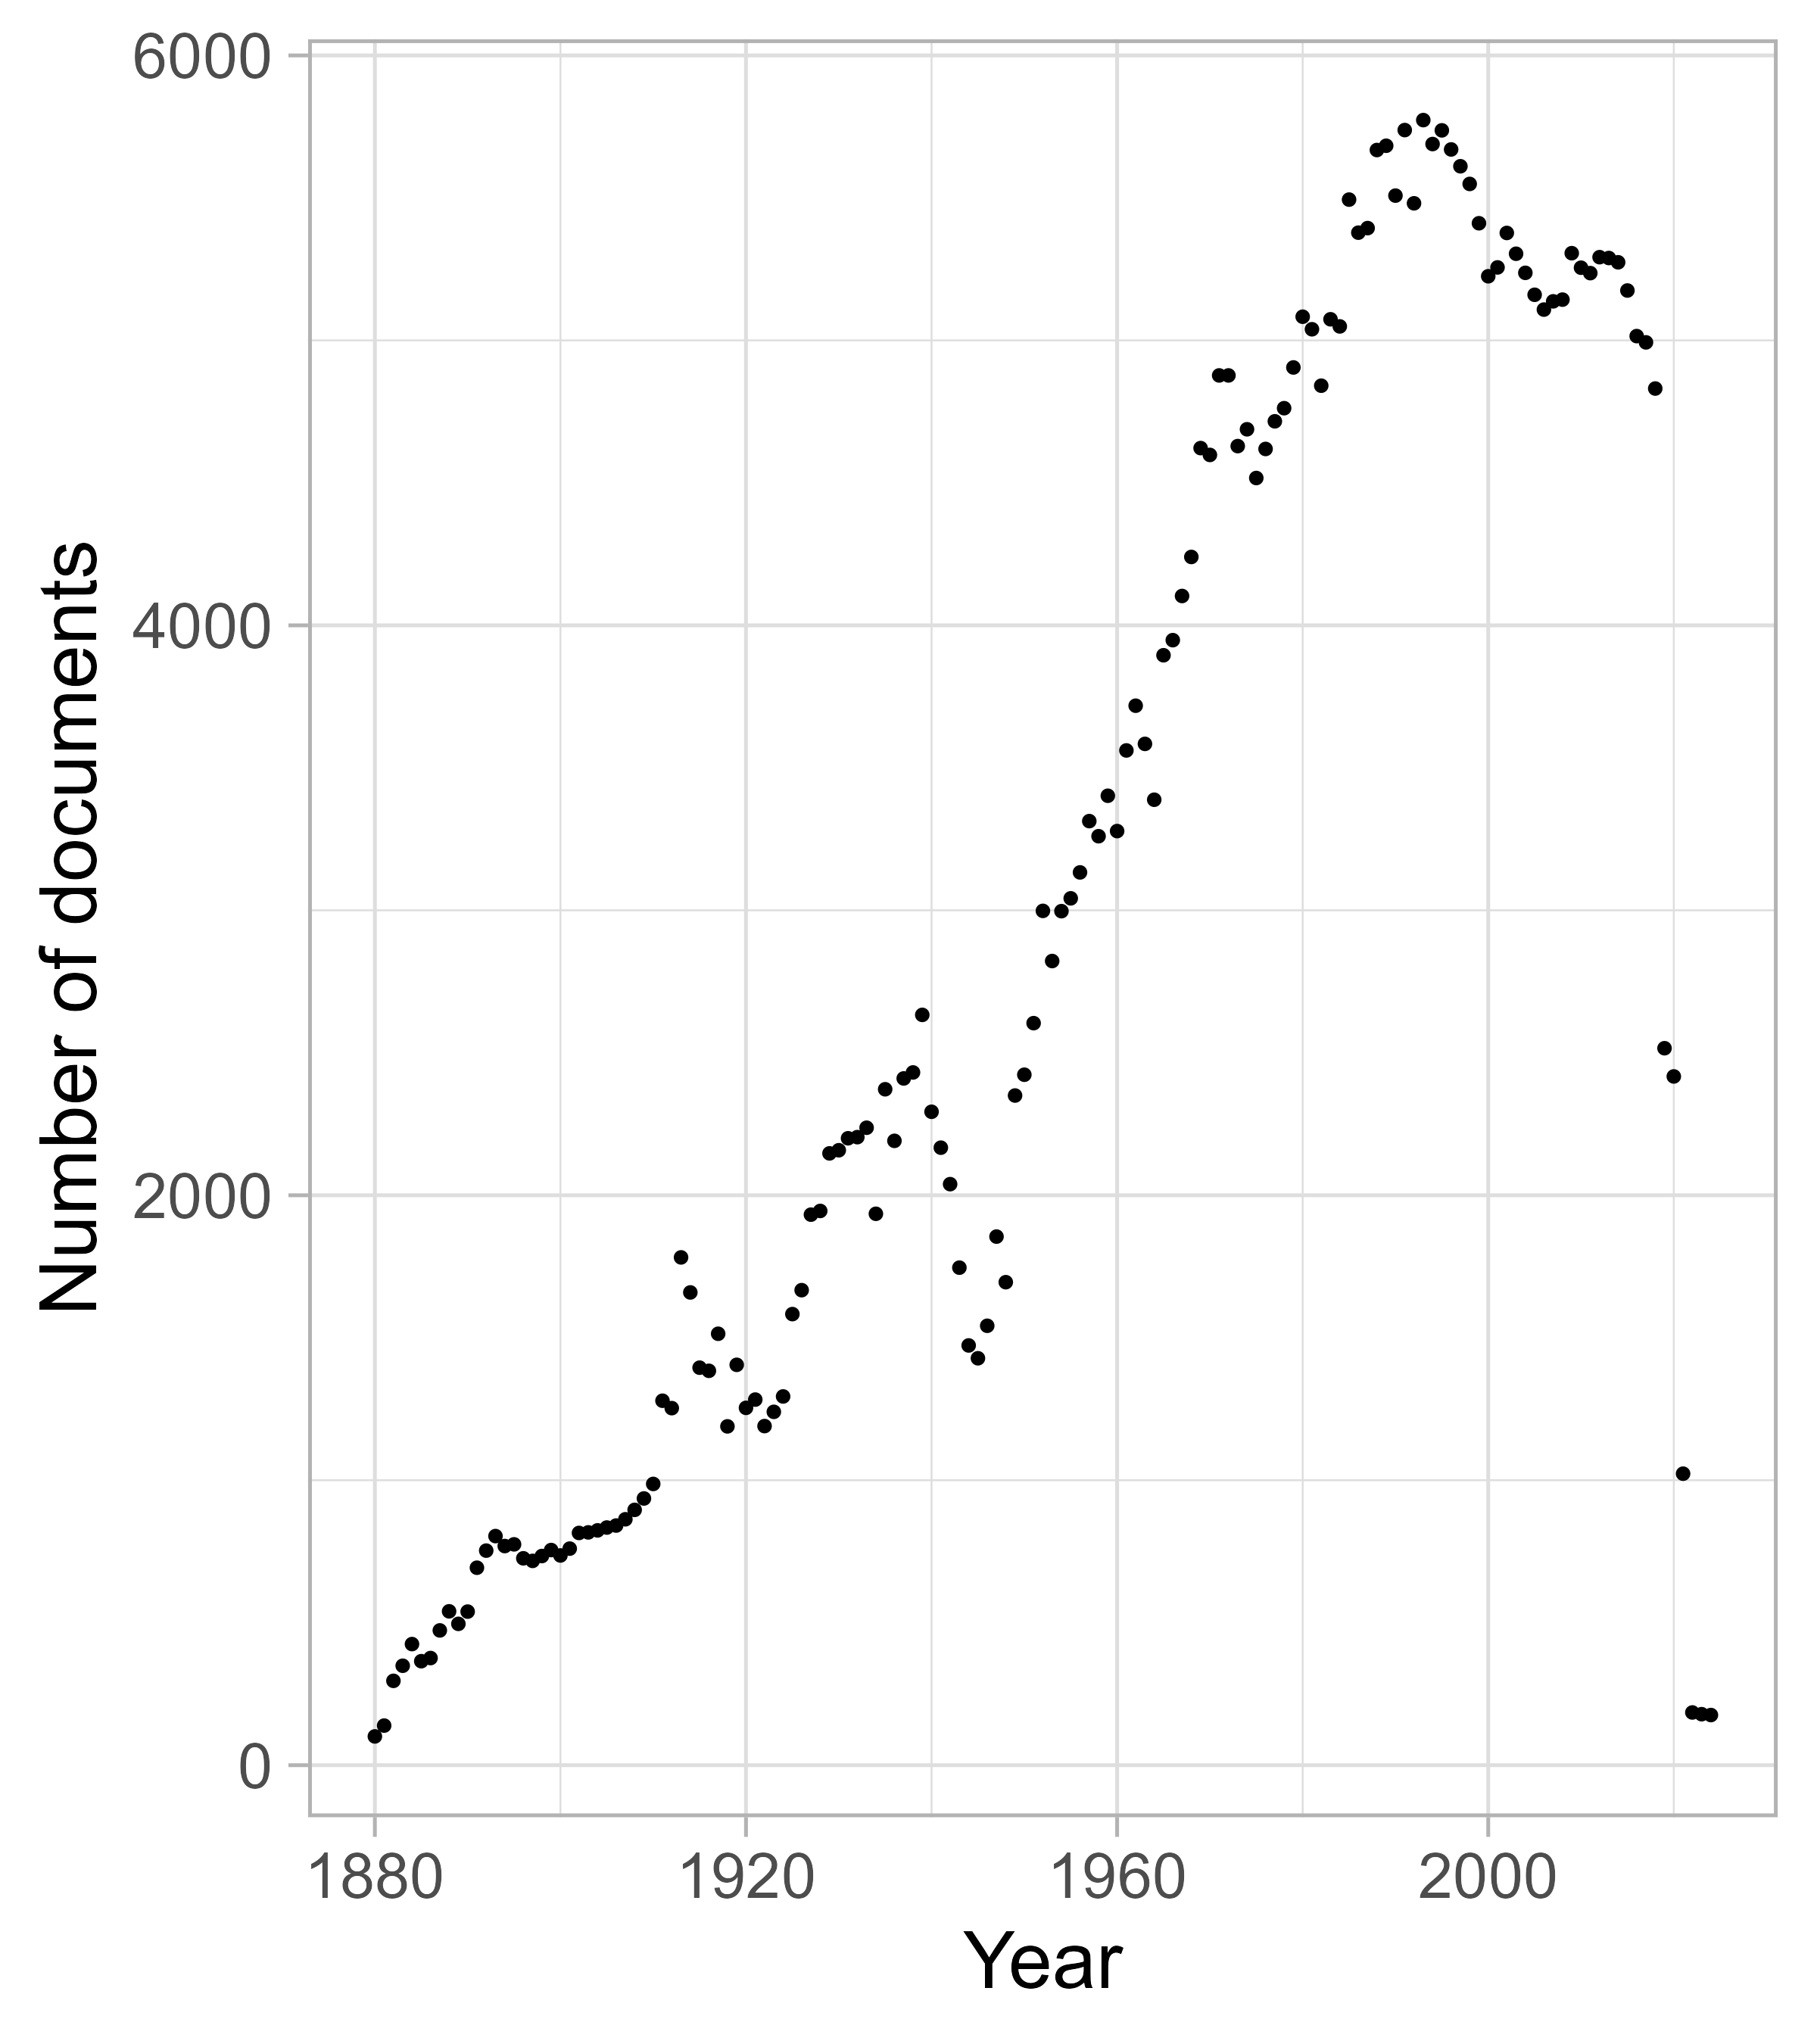
\includegraphics[width=0.9\linewidth,height=\textheight,keepaspectratio]{images/documents_distribution_fulltext_database.png}

}

\subcaption{\label{fig-jstordistribution_a}Documents}

\end{minipage}%
%
\begin{minipage}{0.50\linewidth}

\centering{

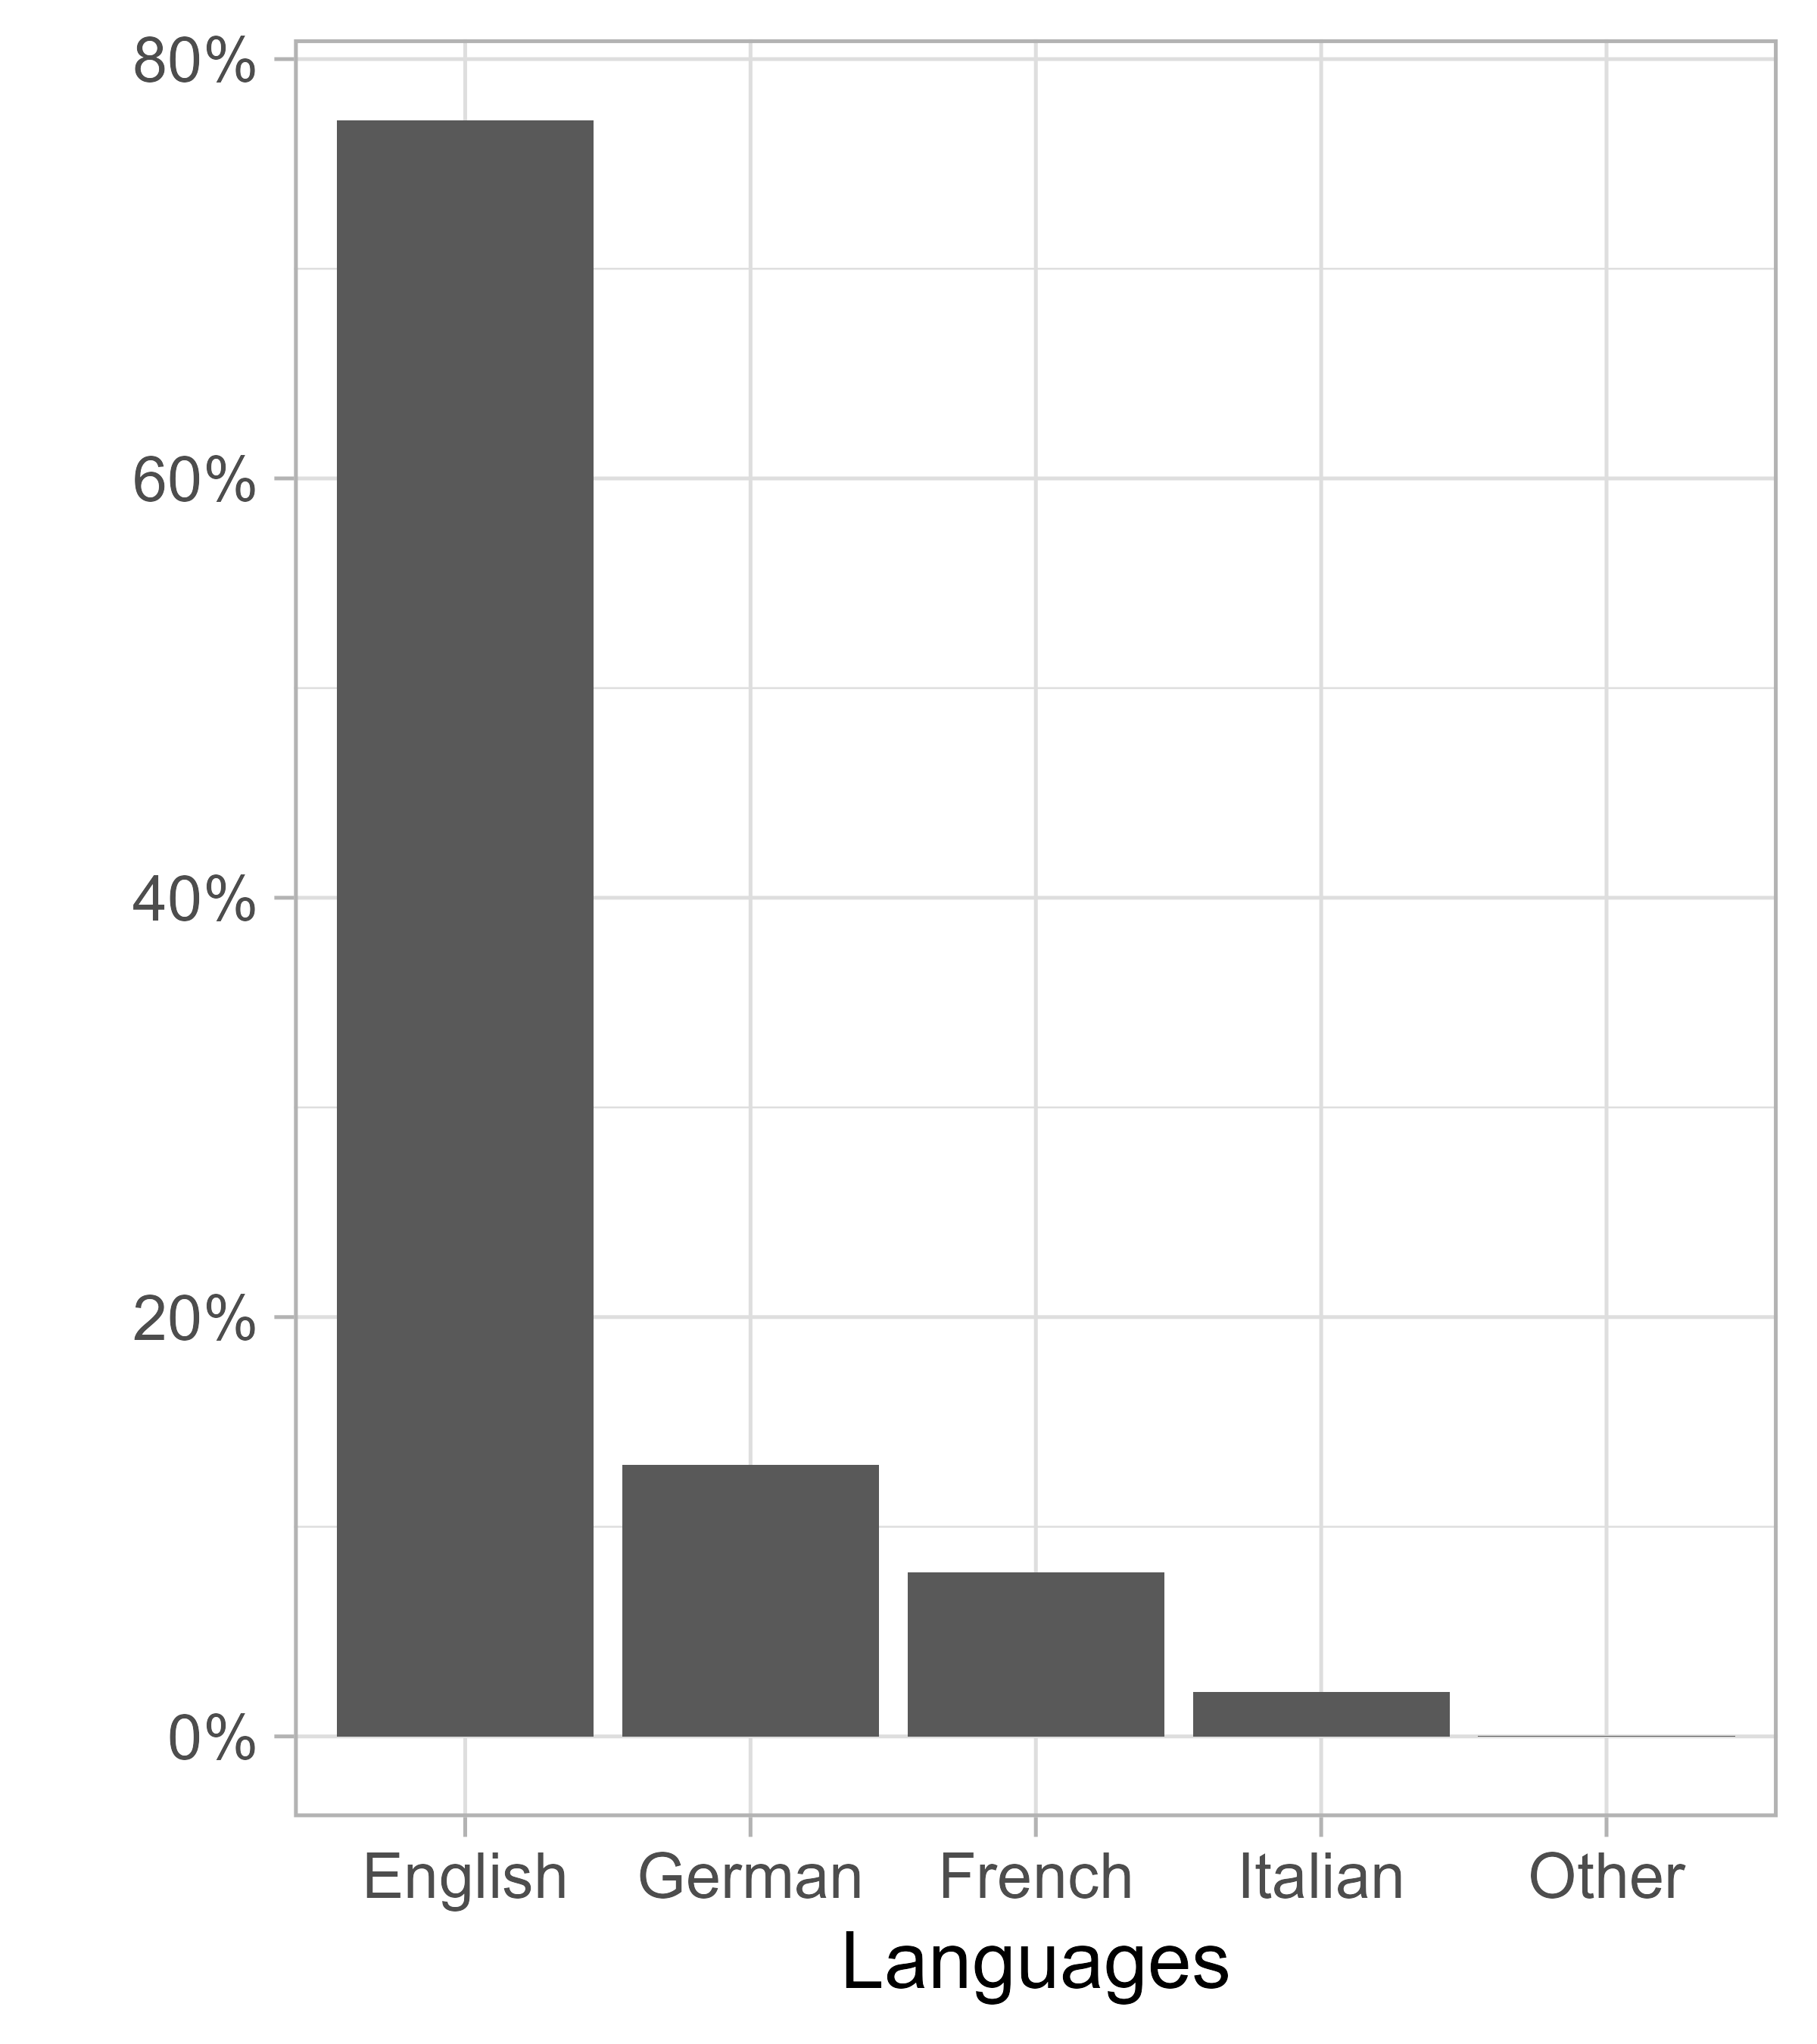
\includegraphics[width=0.9\linewidth,height=\textheight,keepaspectratio]{images/language_distribution_fulltext_database.png}

}

\subcaption{\label{fig-jstordistribution_b}Languages}

\end{minipage}%

\caption{\label{fig-distribution}General statistics of the JSTOR
full-text database}

\end{figure}%

\begin{figure}

\centering{

\pandocbounded{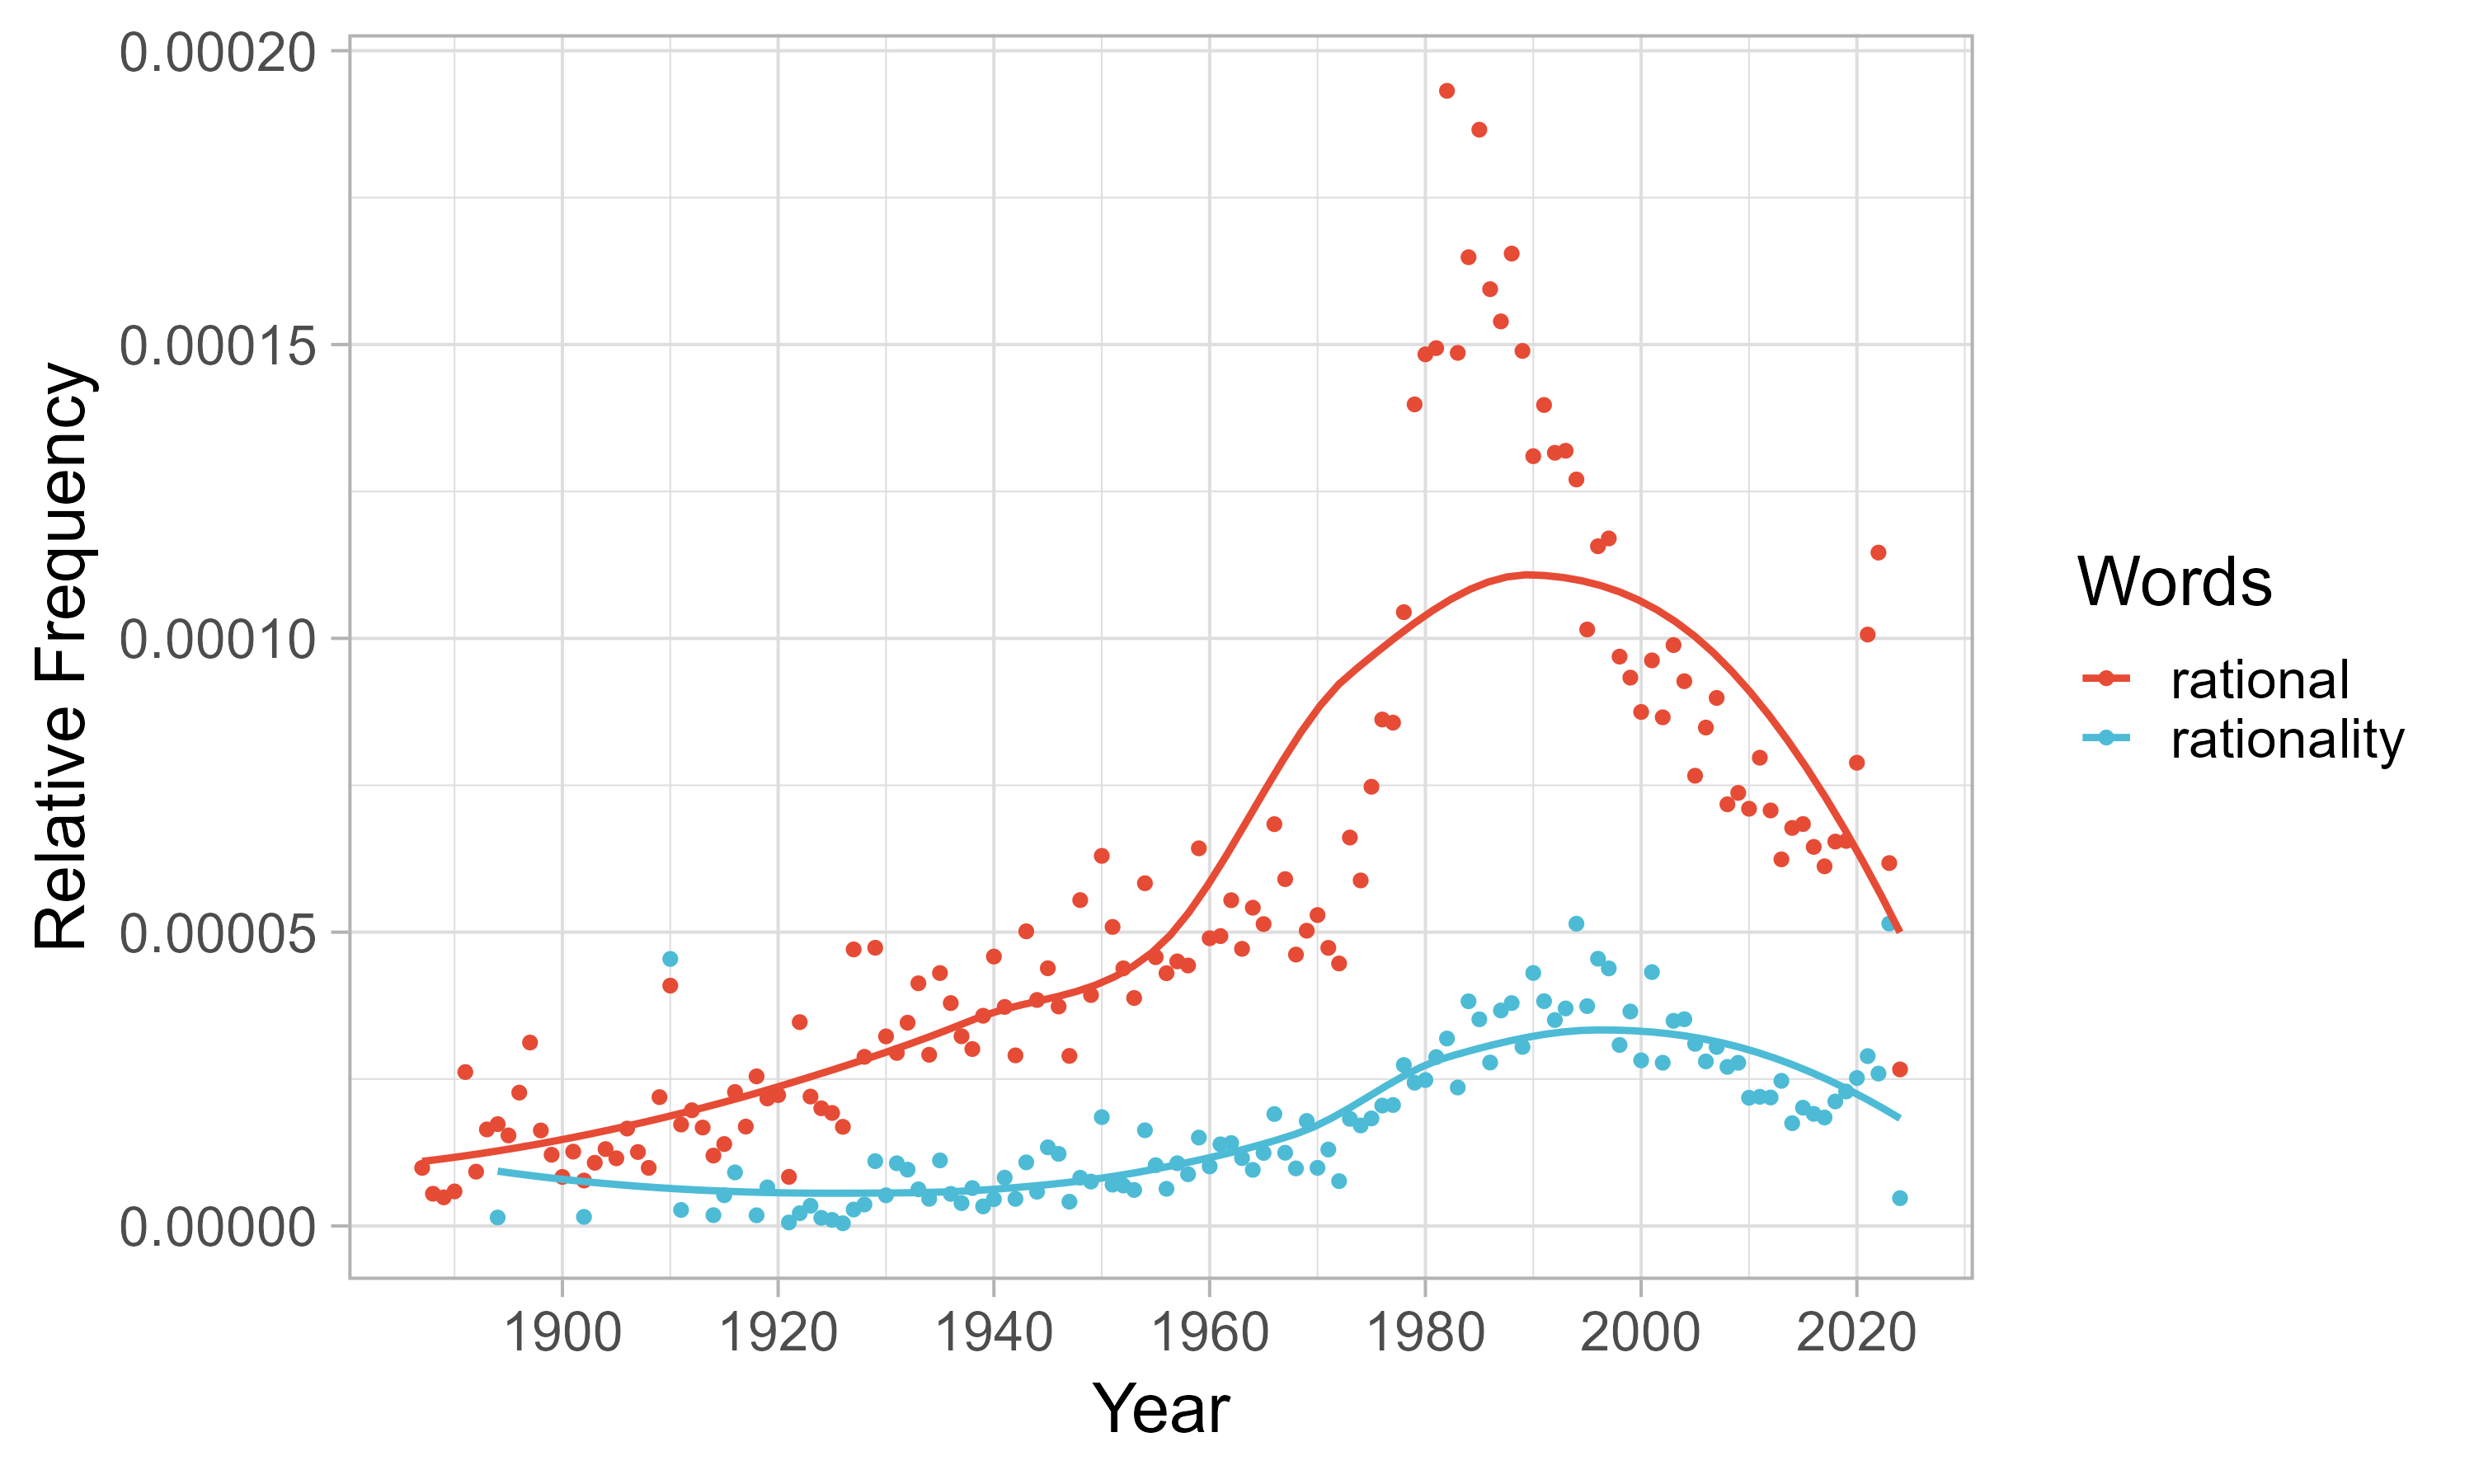
\includegraphics[keepaspectratio]{images/relative_freq_rationality_and_rational.png}}

}

\caption{\label{fig-relative-frequency}Relative frequency of terms
``rational'' and ``rationality'' in the jstor database}

\end{figure}%

\begin{figure}

\centering{

\pandocbounded{\includegraphics[keepaspectratio]{images/top_neighbor_words_both.png}}

}

\caption{\label{fig-co-occurence}Most frequent neighbor terms of
``rational'' and ``rationality'' by decade}

\end{figure}%

\begin{figure}

\centering{

\pandocbounded{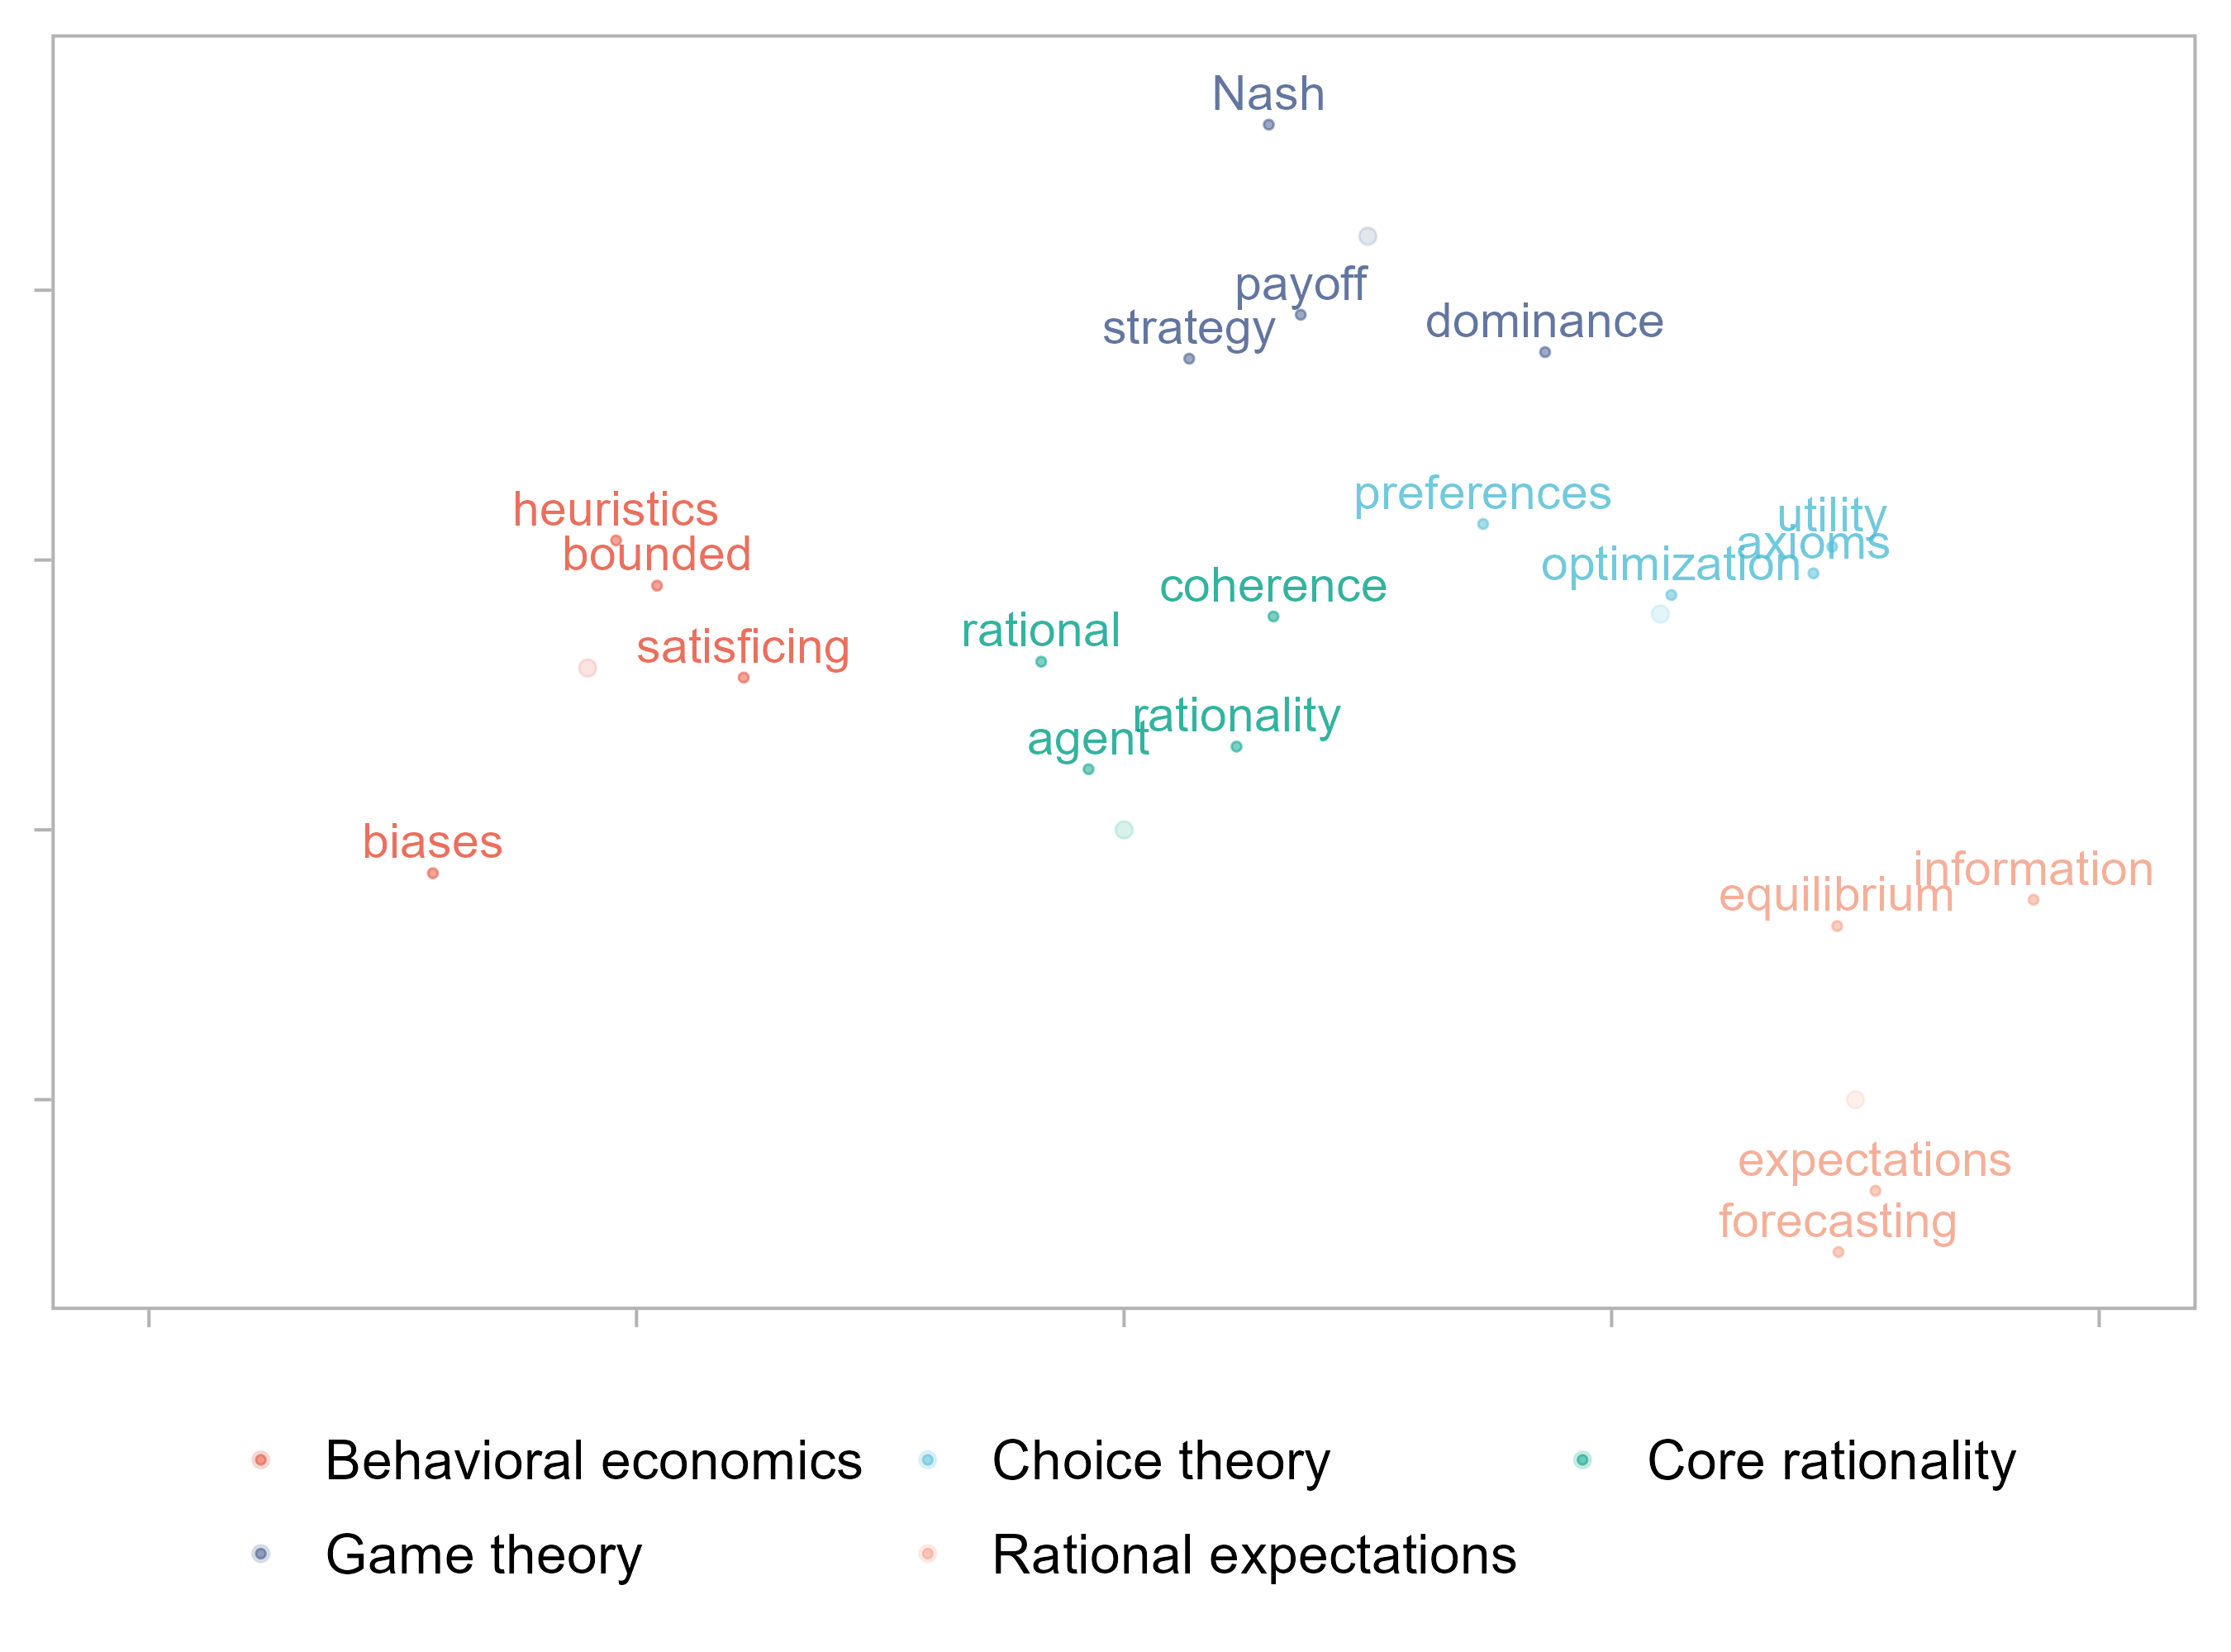
\includegraphics[keepaspectratio]{images/fake_semantic_space_words_in_2D.png}}

}

\caption{\label{fig-embedding-example}Illustration of word embeddings in
two dimension space}

\end{figure}%

\begin{table}

\caption{\label{tbl-example-comparison}The three closest sentences to
representative vectors of rationality for selected years.}

\centering{

\centering\begingroup\fontsize{7}{9}\selectfont

\begin{threeparttable}
\begin{tabular}[t]{>{\centering\arraybackslash}p{1.2cm}>{\raggedright\arraybackslash}p{10cm}>{\centering\arraybackslash}p{1.2cm}}
\toprule
Year & Sentence & Cosine similarity\\
\midrule
1925 & The motive power to action, to the pursuit of practical ends, good or bad, lies not in intelligence, but in feeling, instinct, and impulse; and the higher, sustained ends which man pursues depend upon his sentiments or permanent interests. & 0.653\\
1925 & Our interest in simplicity and definiteness has at some point to yield to other interests with which it comes into conflict and which cannot be denied. & 0.625\\
1925 & That is, we have to recognize men's conscious interests not only as existent and causal and explanatory in the descriptive, scientific sense, as data in a uniformity of sequence, but as causal and explanatory in a further sense, to which it is difficult if not impossible to give clear expression in language. & 0.619\\
1950 & Where these are precisely stated at all, they usually assume a business man who is perfectly rational (apart from " waves of sentiment " which may reach him from outside), and whose brain, apparently of great capacity, is capable of performing integrations and of founding judgments upon a calculation of a mathematical expectation. & 0.678\\
1950 & Rationalization on the societal level, rather than the industrial level we are accustomed to think of in this connection, calls for a different order of engineer and for a different order of techniques. & 0.655\\
\addlinespace
1950 & Even completely rational behavior, therefore, represents a system of discontinuous functions, in which a quantity or price change has to be much larger than "infinitesimal" before it acts as a stimulus producing response. & 0.650\\
1975 & Howard, N. Paradoxes of Rationality. & 0.722\\
1975 & A more fundamental question concerns the way in which the private sector form their expectations ; if they are 'rationalthat is based on information at least as good as the authorities', then the grounds for discretionary intervention by the authorities are greatly diminished. & 0.720\\
1975 & Thus in genera1 rationality dues not mean the use of unbiasedpredictors. & 0.713\\
2000 & Our aim was to provide on overall picture how decisions of boundedly rational decision makers emerge. & 0.808\\
\addlinespace
2000 & An important approach to discussing the notion of rationality may be found in . & 0.806\\
2000 & For further discussion of the informal rationality constraint's connection to decision-theoretic conceptions of rationality, see Carroll (1999). & 0.804\\
\bottomrule
\end{tabular}
\begin{tablenotes}
\item \textit{Note: } 
\item Cosine similarities from the representative vectors; three nearest sentences per selected year.
\end{tablenotes}
\end{threeparttable}
\endgroup{}

}

\end{table}%

\begin{figure}[H]

{\centering \pandocbounded{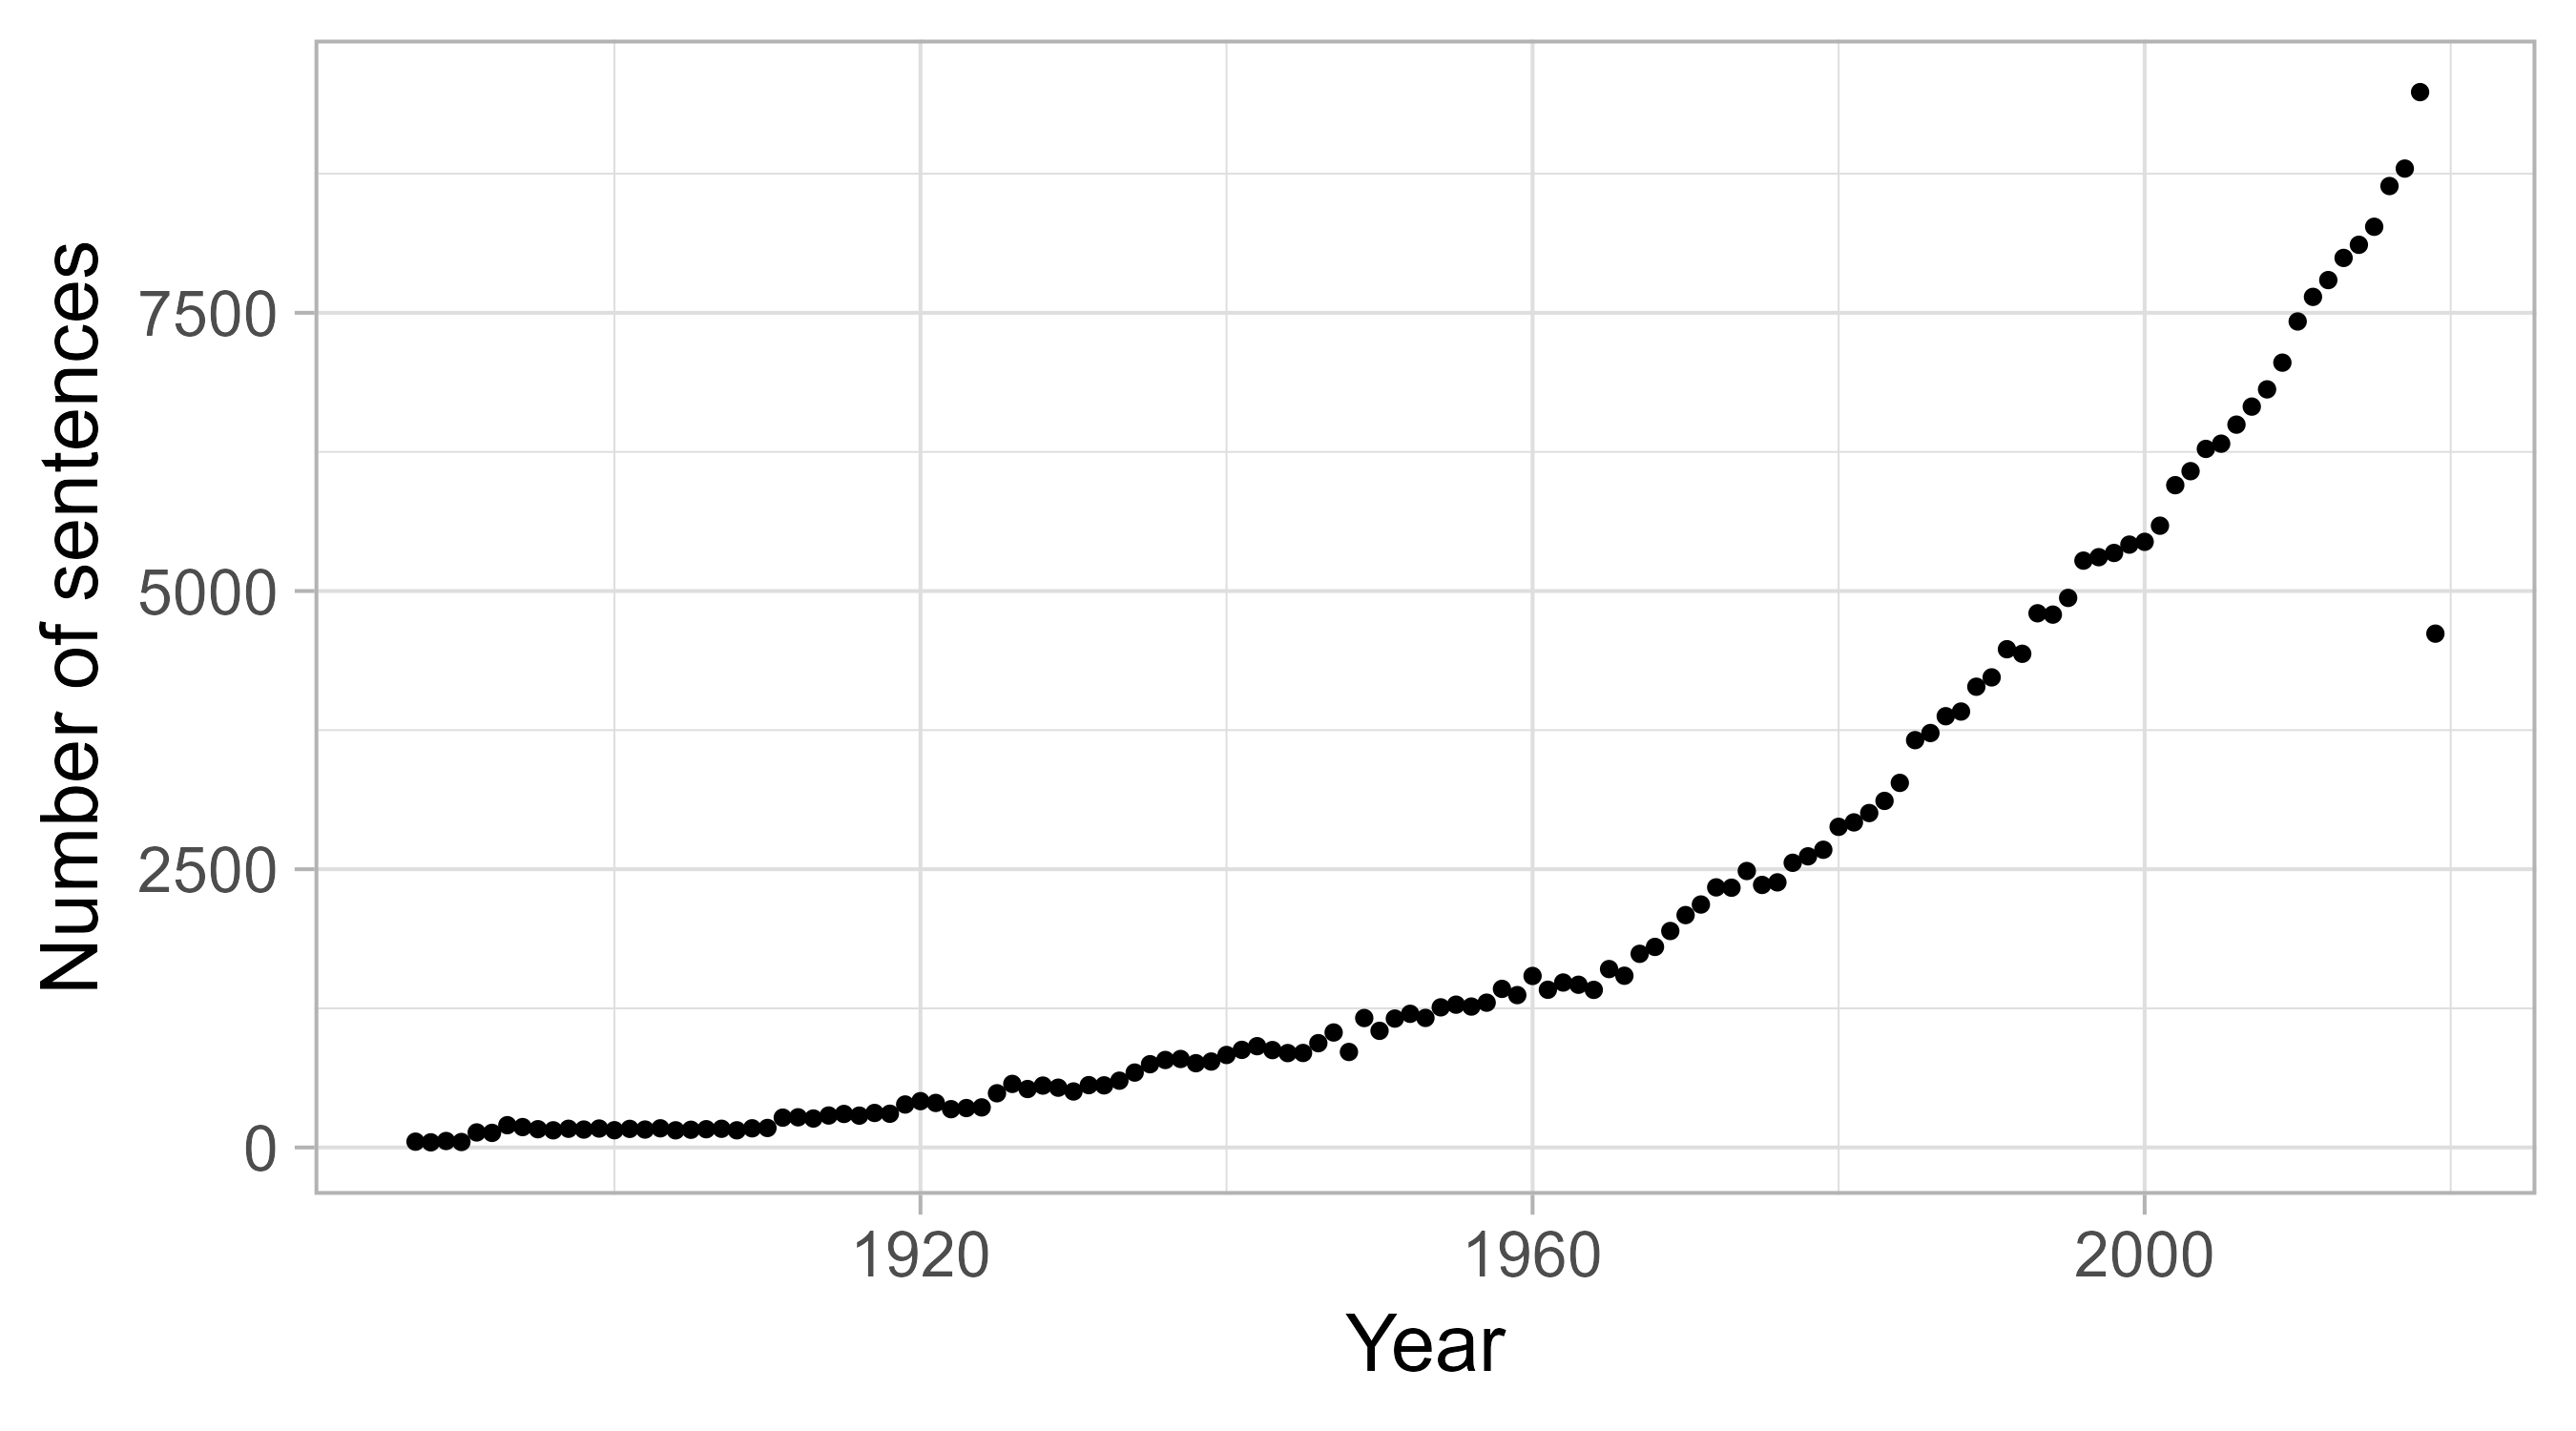
\includegraphics[keepaspectratio]{images/distribution_closest_sentences_by_year.png}}

}

\caption{Distribution of cosine similarities to the fake sentence}

\end{figure}%

\begin{landscape}

\begin{figure}

\centering{

\pandocbounded{\includegraphics[keepaspectratio]{images/intertemporal_clusters_alluvial.png}}

}

\caption{\label{fig-llm-alluvial}Alluvial plot of clusters of sentences
about rationality}

\end{figure}%

\end{landscape}

\begin{figure}

\centering{

\pandocbounded{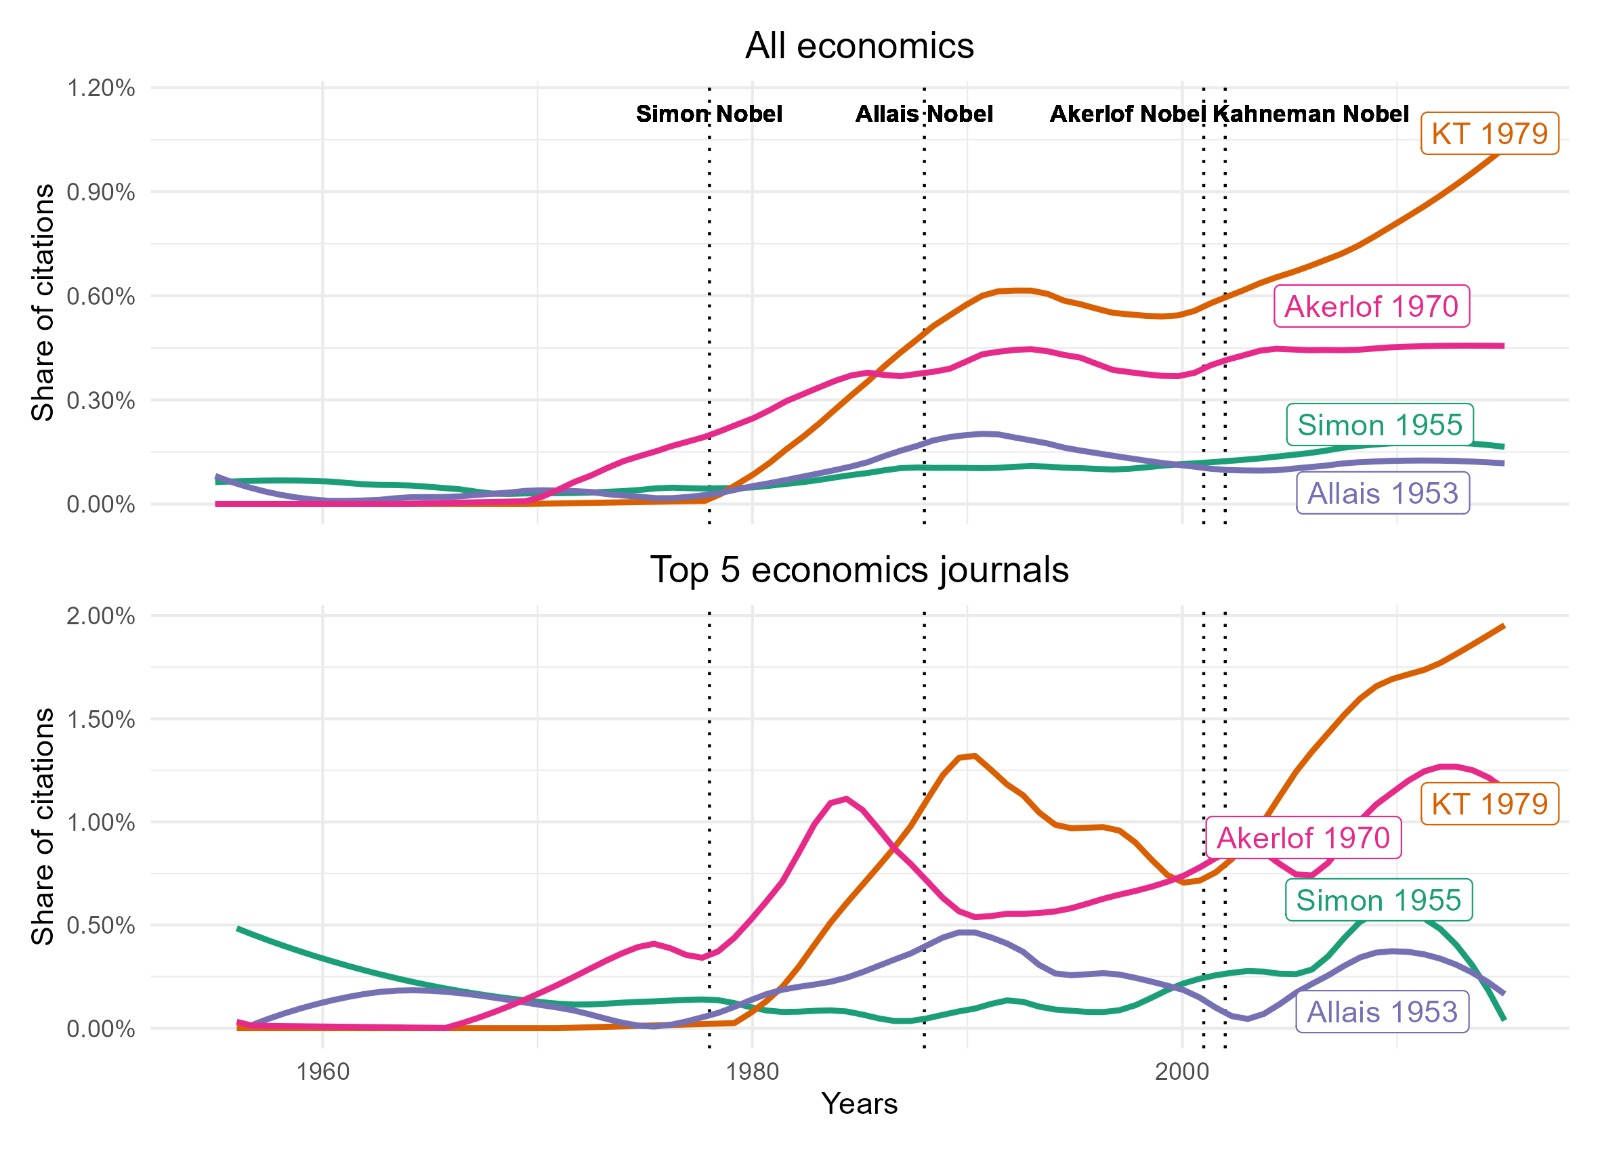
\includegraphics[keepaspectratio]{images/citation_patterns_square.jpg}}

}

\caption{\label{fig-rationality-paper-citations}Relative citation of a
selection of seminal papers on behavioral economics}

\end{figure}%

\begin{landscape}

\begin{figure}

\centering{

\pandocbounded{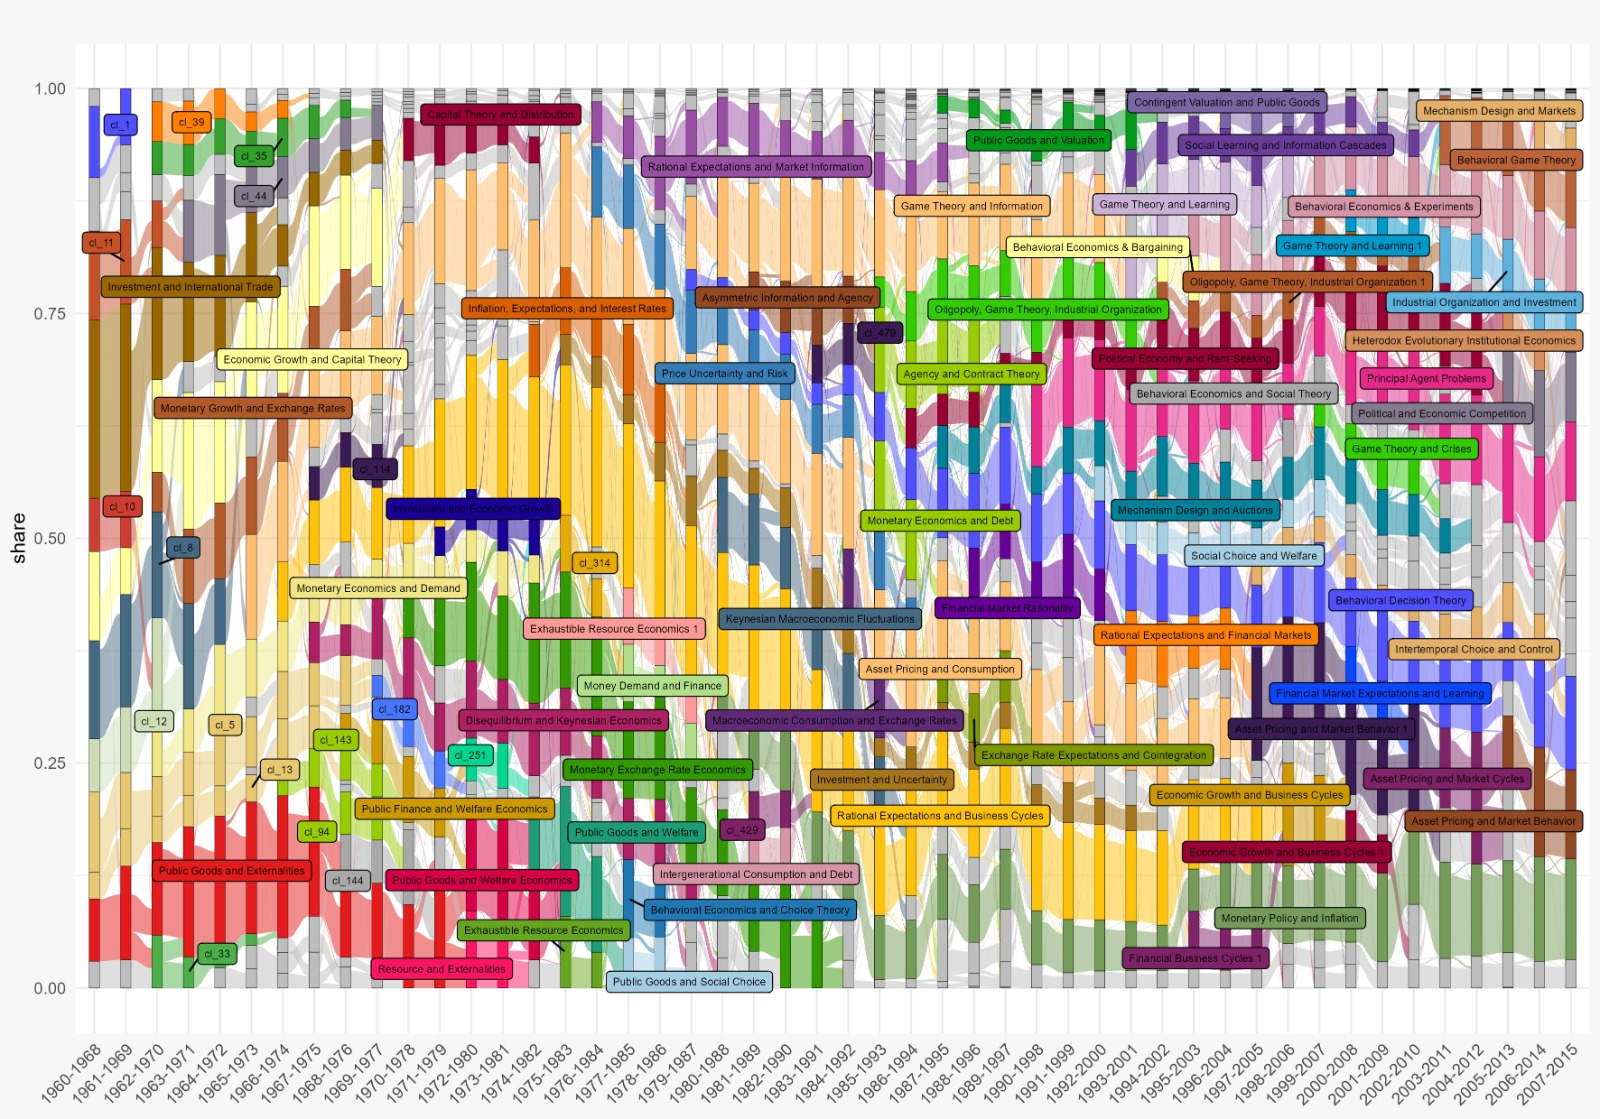
\includegraphics[keepaspectratio]{images/alluvial_network.jpg}}

}

\caption{\label{fig-biblio-alluvial}Alluvial plot of clusters of
sentences about rationality}

\end{figure}%

\end{landscape}

\begin{landscape}

\begin{figure}

\centering{

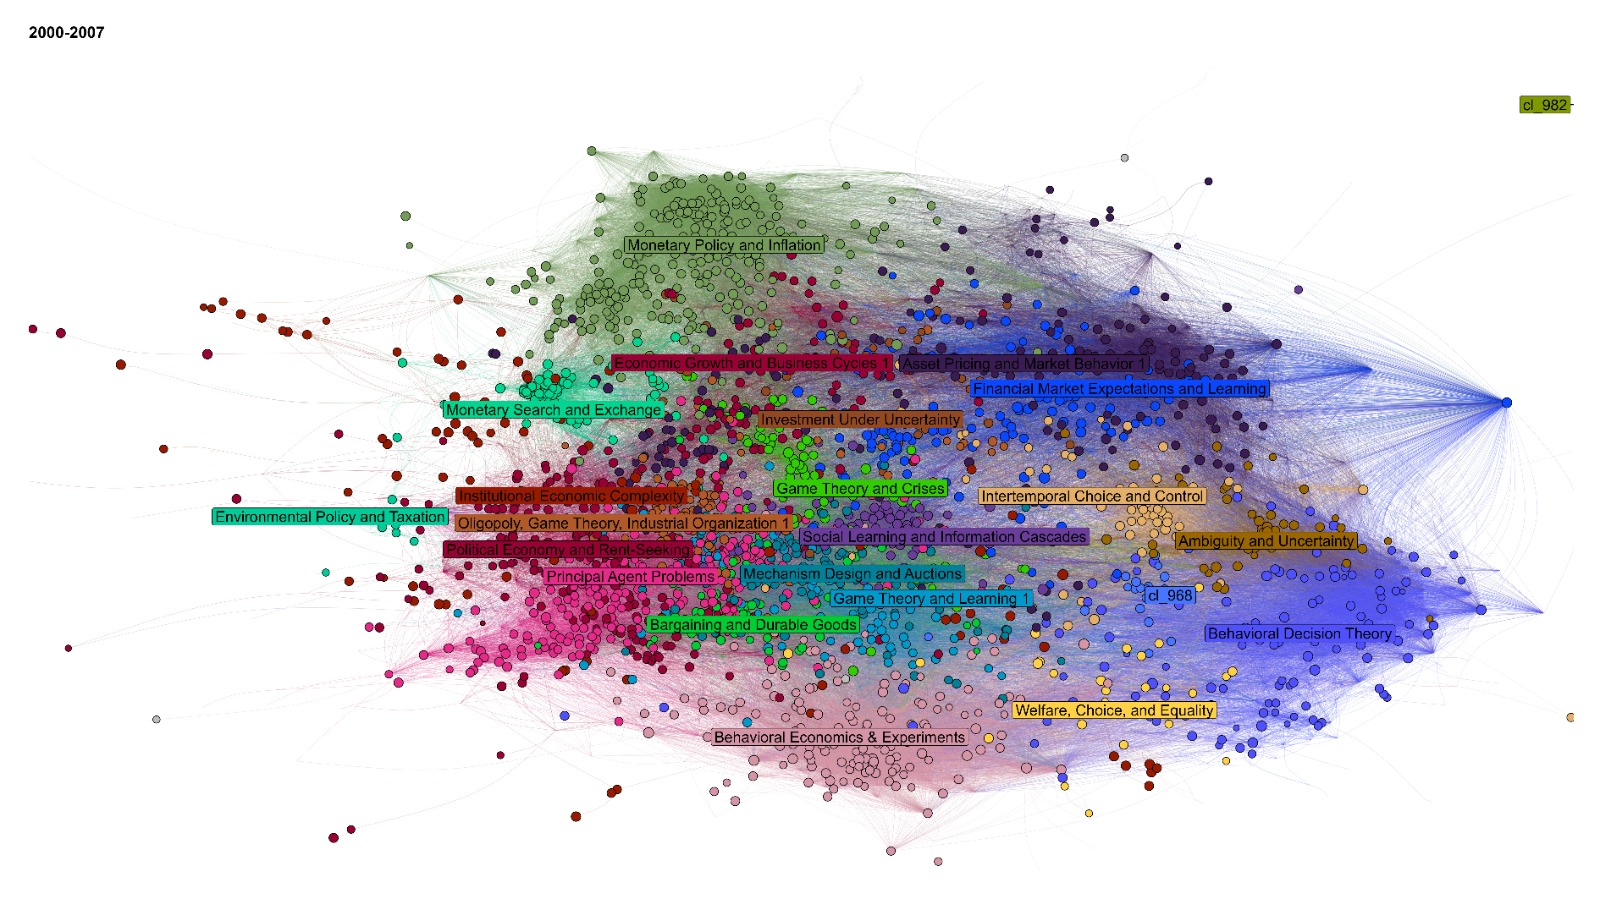
\includegraphics[width=1\linewidth,height=\textheight,keepaspectratio]{images/network_example.jpg}

}

\caption{\label{fig-biblio-network-example}Example of one bibliographic
network representing one horizontal bar of Alluvial
(Figure~\ref{fig-biblio-alluvial})}

\end{figure}%

\end{landscape}

\section*{References}\label{references}
\addcontentsline{toc}{section}{References}

\phantomsection\label{refs}
\begin{CSLReferences}{1}{0}
\bibitem[\citeproctext]{ref-akerlofMarket1970}
Akerlof, George A. 1970. {``The {Market} for "{Lemons}": {Quality
Uncertainty} and the {Market Mechanism}.''} \emph{The Quarterly Journal
of Economics} 84 (3): 488--500. \url{https://doi.org/10.2307/1879431}.

\bibitem[\citeproctext]{ref-allaisComportementHommeRationnel1953}
Allais, M. 1953. {``Le {Comportement} de l'{Homme Rationnel} Devant Le
{Risque}: {Critique} Des {Postulats} Et {Axiomes} de l'{Ecole
Americaine}.''} \emph{Econometrica} 21 (4): 503.
\url{https://doi.org/10.2307/1907921}.

\bibitem[\citeproctext]{ref-ambrosinoWhat2018}
Ambrosino, Angela, Mario Cedrini, John B. Davis, Stefano Fiori, Marco
Guerzoni, and Massimiliano Nuccio. 2018. {``What Topic Modeling Could
Reveal about the Evolution of Economics.''} \emph{Journal of Economic
Methodology} 25 (4): 329--48.
\url{https://doi.org/10.1080/1350178X.2018.1529215}.

\bibitem[\citeproctext]{ref-arrowExistence1954}
Arrow, Kenneth J, and Gerard Debreu. 1954. {``Existence of an
Equilibrium for a Competitive Economy.''} \emph{Econometrica: Journal of
the Econometric Society}, 265--90.

\bibitem[\citeproctext]{ref-backhouseAge2017}
Backhouse, Roger E., and Béatrice Cherrier. 2017. {``The {Age} of the
{Applied Economist}: {The Transformation} of {Economics} Since the
1970s.''} \emph{History of Political Economy} 49 (Supplement): 1--33.
\url{https://doi.org/10.1215/00182702-4166239}.

\bibitem[\citeproctext]{ref-barroPositive1983}
Barro, Robert J., and David B. Gordon. 1983. {``A {Positive Theory} of
{Monetary Policy} in a {Natural Rate Model}.''} \emph{Journal of
Political Economy} 91 (4): 589--610.
\url{https://www.jstor.org/stable/1831069}.

\bibitem[\citeproctext]{ref-beckerIrrational1962}
Becker, Gary S. 1962. {``Irrational {Behavior} and {Economic Theory}.''}
\emph{Journal of Political Economy} 70 (1): 1--13.
\url{https://www.jstor.org/stable/1827018}.

\bibitem[\citeproctext]{ref-boumansEngineering2020}
Boumans, Marcel. 2020. {``The {Engineering Tools That Shaped} the
{Rational Expectations Revolution}.''} \emph{History of Political
Economy} 52 (S1): 143--67.
\url{https://doi.org/10.1215/00182702-8717960}.

\bibitem[\citeproctext]{ref-budiUnderstanding2023}
Budi, Indra, and Yaniasih Yaniasih. 2023. {``Understanding the Meanings
of Citations Using Sentiment, Role, and Citation Function
Classifications.''} \emph{Scientometrics} 128 (1): 735--59.
\url{https://doi.org/10.1007/s11192-022-04567-4}.

\bibitem[\citeproctext]{ref-chernoffRational1954}
Chernoff, Herman. 1954. {``Rational {Selection} of {Decision
Functions}.''} \emph{Econometrica} 22 (4): 422--43.
\url{https://doi.org/10.2307/1907435}.

\bibitem[\citeproctext]{ref-cherrierQuantitative2018}
Cherrier, Beatrice, and Andrej Svorenčík. 2018. {``The Quantitative Turn
in the History of Economics: Promises, Perils and Challenges.''}
\emph{Journal of Economic Methodology} 0 (0): 1--11.
\url{https://doi.org/10.1080/1350178X.2018.1529217}.

\bibitem[\citeproctext]{ref-coaseProblem1960}
Coase, Ronald H. 1960. {``The {Problem} of {Social Cost}.''}
\emph{Journal of Law and Economics} 3: 1.

\bibitem[\citeproctext]{ref-cyertRational1974}
Cyert, Richard M., and Morris H. DeGroot. 1974. {``Rational
{Expectations} and {Bayesian Analysis}.''} \emph{Journal of Political
Economy} 82 (3): 521--36. \url{https://www.jstor.org/stable/1829843}.

\bibitem[\citeproctext]{ref-cyertCompetition1969}
Cyert, Richard M., and Kenneth D. George. 1969. {``Competition,
{Growth}, and {Efficiency}.''} \emph{The Economic Journal} 79 (313):
23--41. \url{https://doi.org/10.2307/2229627}.

\bibitem[\citeproctext]{ref-dasilvaLucass2017}
da Silva, R. D. F. 2017. {``Lucas's {Research} in the {Late} 1960s and
the {Natural Rate} of {Unemployment}.''} \emph{History of Political
Economy} 49 (1): 137--59.
\url{https://doi.org/10.1215/00182702-3777194}.

\bibitem[\citeproctext]{ref-delceyEfficient2023}
Delcey, Thomas, and Francesco Sergi. 2023. {``The Efficient Market
Hypothesis and Rational Expectations Macroeconomics. {How} Did They Meet
and Live (Happily) Ever After?''} \emph{The European Journal of the
History of Economic Thought} 30 (1): 86--116.
\url{https://doi.org/10.1080/09672567.2022.2108869}.

\bibitem[\citeproctext]{ref-dornbuschExpectations1976}
Dornbusch, Rudiger. 1976. {``Expectations and {Exchange Rate
Dynamics}.''} \emph{Journal of Political Economy} 84 (6): 1161--76.
\url{https://www.jstor.org/stable/1831272}.

\bibitem[\citeproctext]{ref-duarteRise2025}
Duarte, Pedro G. 2025. {``The {Rise} of the {Rational Expectations
Hypothesis}.''} In.

\bibitem[\citeproctext]{ref-duarteFeasible2009}
Duarte, Pedro Garcia. 2009. {``A {Feasible} and {Objective Concept} of
{Optimal Monetary Policy}: {The Quadratic Loss Function} in the {Postwar
Period}.''} \emph{History of Political Economy} 41 (1): 1--55.

\bibitem[\citeproctext]{ref-duppeFinding2014}
Düppe, Till, and E. Roy Weintraub. 2014. \emph{Finding Equilibrium:
{Arrow}, {Debreu}, {McKenzie} and the Problem of Scientific Credit}.
Princeton: Princeton University Press.

\bibitem[\citeproctext]{ref-earlPrinciples2022}
Earl, Peter E. 2022. \emph{Principles of Behavioral Economics: Bringing
Together Old, New and Evolutionary Approaches}. Cambridge, United
Kingdom New York, NY Port Melbourne, VIC New Delhi Singapore: Cambridge
University Press. \url{https://doi.org/10.1017/9781009091053}.

\bibitem[\citeproctext]{ref-edwardsQuantitative2018}
Edwards, José, Yann Giraud, and Christophe Schinckus. 2018. {``A
Quantitative Turn in the Historiography of Economics?''} \emph{Journal
of Economic Methodology} 25 (4): 283--90.
\url{https://doi.org/10.1080/1350178X.2018.1529133}.

\bibitem[\citeproctext]{ref-ellsbergTheory1956}
Ellsberg, Daniel. 1956. {``Theory of the {Reluctant Duelist}.''}
\emph{American Economic Review} 46 (5): 909--23.
\url{https://www.jstor.org/stable/1811911}.

\bibitem[\citeproctext]{ref-ericksonHow2013}
Erickson, Paul, Judy L. Klein, Lorraine Daston, Rebecca Lemov, Thomas
Sturm, and Michael D. Gordin. 2013. \emph{{How Reason Almost Lost Its
Mind -- The Strange Career of Cold War Rationality}}. Reprint.
University of Chicago Press.

\bibitem[\citeproctext]{ref-ericssonWorld2015}
Ericsson, Neil. 2015. \emph{The {World} the {Game Theorists Made}}.

\bibitem[\citeproctext]{ref-fairCriticism1978}
Fair, Ray C. 1978. {``A {Criticism} of {One Class} of {Macroeconomic
Models} with {Rational Expectations}.''} \emph{Journal of Money, Credit
and Banking} 10 (4): 411. \url{https://doi.org/10.2307/1991572}.

\bibitem[\citeproctext]{ref-firthStudies1957}
Firth, John Rupert. 1957. \emph{Studies in Linguistic Analysis}. Basil
Blackwell Oxford.

\bibitem[\citeproctext]{ref-friedmanUtility1948}
Friedman, Milton, and L. J. Savage. 1948. {``The {Utility Analysis} of
{Choices Involving Risk}.''} \emph{Journal of Political Economy} 56 (4):
279--304. \url{https://www.jstor.org/stable/1826045}.

\bibitem[\citeproctext]{ref-friedmanExpectedUtility1952}
---------. 1952. {``The {Expected-Utility Hypothesis} and the
{Measurability} of {Utility}.''} \emph{Journal of Political Economy} 60
(6): 463--74. \url{https://www.jstor.org/stable/1825271}.

\bibitem[\citeproctext]{ref-georgescu-roegenChoice1954}
Georgescu-Roegen, Nicholas. 1954. {``Choice, {Expectations} and
{Measurability}.''} \emph{The Quarterly Journal of Economics} 68 (4):
503--34. \url{https://doi.org/10.2307/1881875}.

\bibitem[\citeproctext]{ref-giocoliModeling2003}
Giocoli, Nicola. 2003. \emph{Modeling Rational Agents: From Interwar
Economics to Early Modern Game Theory}. Cheltenham, UK Northampton, MA:
Edward Elgar Publishing.

\bibitem[\citeproctext]{ref-goutsmedtQuantitative2023}
Goutsmedt, Aurélien, François Claveau, and Catherine Herfeld. 2023.
{``Quantitative and {Computational Approaches} in the {Social Studies}
of {Economics}.''} \emph{Oeconomia - History, Methodology, Philosophy}
13 (2): 147--61.
https://doi.org/\url{https://journals.openedition.org/oeconomia/15799}.

\bibitem[\citeproctext]{ref-goutsmedtReacting2019}
Goutsmedt, Aurélien, Erich Pinzón-Fuchs, Matthieu Renault, and Francesco
Sergi. 2019. {``Reacting to the {Lucas Critique}: {The Keynesians}'
{Pragmatic Replies}.''} \emph{History of Political Economy} 51 (3):
533--56.
https://doi.org/\url{https://read.dukeupress.edu/hope/article-abstract/51/3/535/137809/Reacting-to-the-Lucas-CritiqueThe-Keynesians?redirectedFrom=fulltext}.

\bibitem[\citeproctext]{ref-goutsmedtIndependent2023}
Goutsmedt, Aurélien, and Alexandre Truc. 2023. {``An {Independent
European Macroeconomics}? {A History} of {European Macroeconomics}
Through the {Lens} of the {European Economic Review}.''} \emph{European
Economic Review} 158: 104559.
\url{https://doi.org/10.1016/j.euroecorev.2023.104559}.

\bibitem[\citeproctext]{ref-grimmerText2022}
Grimmer, Justin, Margaret E. Roberts, and Brandon M. Stewart. 2022.
\emph{Text {As Data}: {A New Framework} for {Machine Learning} and the
{Social Sciences}}. Princeton: Princeton University Press.

\bibitem[\citeproctext]{ref-grossmanImpossibility1980}
Grossman, Sanford J., and Joseph E. Stiglitz. 1980. {``On the
Impossibility of Informationally Efficient Markets.''} \emph{American
Economic Review} 70 (3): 393--408.
\url{https://www.jstor.org/stable/1805228}.

\bibitem[\citeproctext]{ref-guldiDangerous2023}
Guldi, Jo. 2023. \emph{The {Dangerous Art} of {Text Mining}: {A
Methodology} for {Digital History}}. 1st ed. Cambridge University Press.
\url{https://doi.org/10.1017/9781009263016}.

\bibitem[\citeproctext]{ref-handsNormative2015}
Hands, D. Wade. 2015. {``Normative Rational Choice Theory: Past,
Present, and Future.''} \emph{Present, and Future (March 2015)}.

\bibitem[\citeproctext]{ref-herfeldMathematical2017}
Herfeld, Catherine. 2017. {``Between Mathematical Formalism, Normative
Choice Rules, and the Behavioural Sciences: {The} Emergence of Rational
Choice Theories in the Late 1940s and Early 1950s.''} \emph{The European
Journal of the History of Economic Thought}, November.

\bibitem[\citeproctext]{ref-herfeldTheories2018}
---------. 2018. {``From Theories of Human Behavior to Rules of Rational
Choice: Tracing a Normative Turn at the {Cowles Commission},
1943--54.''} \emph{History of Political Economy} 50 (1): 1--48.

\bibitem[\citeproctext]{ref-heukelomBehavioral2014}
Heukelom, Floris. 2014. \emph{Behavioral Economics: A History}.
Historical Perspectives on Modern Economics. New York, NY, USA:
Cambridge University Press.

\bibitem[\citeproctext]{ref-hicksValue1939}
Hicks, John. 1939. \emph{Value {And Capital}}.

\bibitem[\citeproctext]{ref-hooverNew1988}
Hoover, Kevin D. 1988. \emph{The New Classical Macroeconomics}. Oxford:
Blackwell Publishers.

\bibitem[\citeproctext]{ref-kahnemanProspect1979}
Kahneman, Daniel, and Amos Tversky. 1979. {``Prospect Theory: {An}
Analysis of Decision Under Risk.''} \emph{Econometrica} 47 (2): 363--91.

\bibitem[\citeproctext]{ref-kirtchikRise2024}
Kirtchik, Olessia, and Ivan Boldyrev. 2024. {``{`{Rise} and {Fall}'} of
the {Walrasian Program} in {Economics}: {A Social} and {Intellectual
Dynamics} of the {General Equilibrium Theory}.''} \emph{Journal of the
History of Economic Thought} 46 (1): 1--26.
\url{https://doi.org/10.1017/s1053837222000712}.

\bibitem[\citeproctext]{ref-klaesConceptual2005}
Klaes, Matthias, and Esther-Mirjam Sent. 2005. {``A {Conceptual History}
of the {Emergence} of {Bounded Rationality}.''} \emph{History of
Political Economy} 37 (1): 27--59.
\url{https://doi.org/10.1215/00182702-37-1-27}.

\bibitem[\citeproctext]{ref-kleinCold2015}
Klein, Judy L. 2015. {``The {Cold War Hot House} for {Modeling
Strategies} at the {Carnegie Institute} of {Technology}.''}

\bibitem[\citeproctext]{ref-krepsSequential1982}
Kreps, David M., and Robert Wilson. 1982. {``Sequential {Equilibria}.''}
\emph{Econometrica} 50 (4): 863. \url{https://doi.org/10.2307/1912767}.

\bibitem[\citeproctext]{ref-kydlandRules1977}
Kydland, Finn E., and Edward C. Prescott. 1977. {``Rules {Rather} Than
{Discretion}: {The Inconsistency} of {Optimal Plans}.''} \emph{Journal
of Political Economy} 85 (3): 473--91.
\url{https://www.jstor.org/stable/1830193}.

\bibitem[\citeproctext]{ref-kydlandTime1982}
---------. 1982. {``Time to Build and Aggregate Fluctuations.''}
\emph{Econometrica: Journal of the Econometric Society} 50 (6):
1345--70.

\bibitem[\citeproctext]{ref-leibensteinAllocative1966}
Leibenstein, Harvey. 1966. {``Allocative {Efficiency} Vs.
"{X-Efficiency}".''} \emph{American Economic Review} 56 (3): 392--415.
\url{https://www.jstor.org/stable/1823775}.

\bibitem[\citeproctext]{ref-lemercierQuantitative2019}
Lemercier, Claire, and Claire Zalc. 2019. \emph{Quantitative Methods in
the Humanities: An Introduction}. Translated by Arthur Goldhammer.
Charlottesville: University of Virginia Press.

\bibitem[\citeproctext]{ref-lucasExpectations1972}
Lucas, Robert E, Jr. 1972. {``Expectations and the Neutrality of
Money.''} \emph{Journal of Economic Theory} 4 (2): 103--24.
\url{https://doi.org/10.1016/0022-0531(72)90142-1}.

\bibitem[\citeproctext]{ref-lucasAsset1978}
Lucas, Robert E. 1978. {``Asset {Prices} in an {Exchange Economy}.''}
\emph{Econometrica} 46 (6): 1429--45.
\url{https://doi.org/10.2307/1913837}.

\bibitem[\citeproctext]{ref-maasMechanical1999}
Maas, Harro. 1999. {``Mechanical {Rationality}: {Jevons} and the
{Making} of {Economic Man}.''} \emph{Studies in History and Philosophy
of Science Part A} 30 (4): 587--619.
\url{https://doi.org/10.1016/S0039-3681(99)00030-8}.

\bibitem[\citeproctext]{ref-marschakRational1950}
Marschak, Jacob. 1950. {``Rational {Behavior}, {Uncertain Prospects},
and {Measurable Utility}.''} \emph{Econometrica} 18 (2): 111--41.
\url{https://doi.org/10.2307/1907264}.

\bibitem[\citeproctext]{ref-mikolovDistributed2013}
Mikolov, Tomas, Ilya Sutskever, Kai Chen, Greg S. Corrado, and Jeff
Dean. 2013. {``Distributed Representations of Words and Phrases and
Their Compositionality.''} \emph{Advances in Neural Information
Processing Systems} 26.

\bibitem[\citeproctext]{ref-millEssays1844}
Mill, John Stuart. 1844. \emph{Essays on {Some Unsettled Questions} of
{Political Economy}}. Project Gutenberg.

\bibitem[\citeproctext]{ref-mirowskiMachine2002}
Mirowski, Philip. 2002. \emph{Machine Dreams: Economics Becomes a Cyborg
Science}. Cambridge ; New York: Cambridge University Press.

\bibitem[\citeproctext]{ref-mitchellRole1916}
Mitchell, Wesley C. 1916. {``The {Role} of {Money} in {Economic
Theory}.''} \emph{The American Economic Review} 6 (1): 140--61.
\url{https://www.jstor.org/stable/1803798}.

\bibitem[\citeproctext]{ref-monginAllais2019}
Mongin, Philippe. 2019. {``The {Allais} Paradox: What It Became, What It
Really Was, What It Now Suggests to Us.''} \emph{Economics and
Philosophy} 35 (3): 423--59.
\url{https://doi.org/10.1017/S0266267118000469}.

\bibitem[\citeproctext]{ref-morettiDistant2013}
Moretti, Franco. 2013. \emph{Distant Reading}. London ; New York: Verso.

\bibitem[\citeproctext]{ref-moscatiRetrospectives2016}
Moscati, Ivan. 2016. {``Retrospectives: How Economists Came to Accept
Expected Utility Theory: The Case of Samuelson and Savage.''}
\emph{Journal of Economic Perspectives} 30 (2): 219--36.

\bibitem[\citeproctext]{ref-moscatiExpected2023}
---------. 2023. \emph{Expected {Utility Theory} and {Beyond}}. 1st ed.
Cambridge: Cambridge University Press.

\bibitem[\citeproctext]{ref-moscatiEllsberg2024}
---------. 2024. {``Ellsberg 1961: {Text}, {Context}, {Influence}.''}
\emph{Decisions in Economics and Finance} 47 (2): 627--53.
\url{https://doi.org/10.1007/s10203-024-00437-1}.

\bibitem[\citeproctext]{ref-muthRational1961}
Muth, John F. 1961. {``Rational {Expectations} and the {Theory} of
{Price Movements}.''} \emph{Econometrica} 29 (3): 315.
\url{https://doi.org/10.2307/1909635}.

\bibitem[\citeproctext]{ref-offerNobel2016}
Offer, Avner, and Gabriel Soderberg. 2016. \emph{The {Nobel Factor}:
{The Prize} in {Economics}, {Social Democracy}, and the {Market Turn}}.
Princeton, NJ: Princeton University Press.

\bibitem[\citeproctext]{ref-perrouxPractice1949}
Perroux, Francois, J. Tinbergen, Jacques Rueff, Evsey D. Domar, E. F.
Lundberg, M. Kalecki, J. Zagorski, and K. Dalal. 1949. {``The {Practice}
of {Economic Planning} and {The Optimum Allocation} of {Resources}:
{Discussion}.''} \emph{Econometrica} 17 (July): 172.
\url{https://doi.org/10.2307/1907305}.

\bibitem[\citeproctext]{ref-reimersSentenceBERT2019}
Reimers, Nils, and Iryna Gurevych. 2019. {``Sentence-{BERT}: {Sentence
Embeddings} Using {Siamese BERT-Networks}.''} arXiv.
\url{https://doi.org/10.48550/arXiv.1908.10084}.

\bibitem[\citeproctext]{ref-rothschildEquilibrium1976}
Rothschild, Michael, and Joseph Stiglitz. 1976. {``Equilibrium in
{Competitive Insurance Markets}: {An Essay} on the {Economics} of
{Imperfect Information}.''} \emph{The Quarterly Journal of Economics} 90
(4): 629--49. \url{https://doi.org/10.2307/1885326}.

\bibitem[\citeproctext]{ref-sargentwallace1975}
Sargent, Thomas J., and Neil Wallace. 1975. {``{`{Rational}'}
{Expectations}, the {Optimal Monetary Instrument}, and the {Optimal
Money Supply Rule}.''} \emph{Journal of Political Economy} 83 (2):
241--54.

\bibitem[\citeproctext]{ref-sargentRational1973}
Sargent, Thomas J, and Neil Wallace. 1973. {``Rational Expectations and
the Dynamics of Hyperinflation.''} \emph{International Economic Review},
328--50.

\bibitem[\citeproctext]{ref-savageFoundations1954}
Savage, Leonard J. 1954. \emph{The {Foundations} of {Statistics}}. New
York: John Wiley.

\bibitem[\citeproctext]{ref-schellingAbandonment1959}
Schelling, T. C. 1959. {``For the {Abandonment} of {Symmetry} in {Game
Theory}.''} \emph{Review of Economics and Statistics} 41 (3): 213--24.
\url{https://doi.org/10.2307/1927448}.

\bibitem[\citeproctext]{ref-seltenReexamination1975}
Selten, R. 1975. {``Reexamination of the Perfectness Concept for
Equilibrium Points in Extensive Games.''} \emph{International Journal of
Game Theory} 4 (1): 25--55. \url{https://doi.org/10.1007/BF01766400}.

\bibitem[\citeproctext]{ref-sent_behavioral_2004}
Sent, E.-M. 2004. {``Behavioral {Economics}: {How Psychology Made Its}
({Limited}) {Way Back Into Economics}.''} \emph{History of Political
Economy} 36 (4): 735--60.
\url{https://doi.org/10.1215/00182702-36-4-735}.

\bibitem[\citeproctext]{ref-sentEvolving1998}
Sent, Esther-Mirjam. 1998. \emph{The {Evolving Rationality} of {Rational
Expectations}: {An Assessment} of {Thomas Sargent}'s {Achievements}}.
Cambridge University Press.

\bibitem[\citeproctext]{ref-sentHow2002}
---------. 2002. {``How ({Not}) to {Influence People}: {The Contrary
Tale} of {John F}. {Muth}.''} \emph{History of Political Economy} 34
(2): 291--319.

\bibitem[\citeproctext]{ref-sentRationality2008}
---------. 2008. {``Rationality, {History} of the {Concept}.''} In
\emph{The {New Palgrave Dictionary} of {Economics}}, edited by Palgrave
Macmillan, 1--11. London: Palgrave Macmillan UK.
\url{https://doi.org/10.1057/978-1-349-95121-5_2834-1}.

\bibitem[\citeproctext]{ref-sentRationality2018}
---------. 2018. {``Rationality and Bounded Rationality: You Can't Have
One Without the Other.''} \emph{The European Journal of the History of
Economic Thought} 25 (6): 1370--86.
\url{https://doi.org/10.1080/09672567.2018.1523206}.

\bibitem[\citeproctext]{ref-sergiStandard2020}
Sergi, Francesco. 2020. {``The Standard Narrative about {DSGE} Models in
Central Banks' Technical Reports.''} \emph{The European Journal of the
History of Economic Thought} 27 (2): 163--93.

\bibitem[\citeproctext]{ref-simonBehavioral1955}
Simon, Herbert A. 1955. {``A {Behavioral Model} of {Rational Choice}.''}
\emph{The Quarterly Journal of Economics} 69 (1): 99--118.
\url{https://doi.org/10.2307/1884852}.

\bibitem[\citeproctext]{ref-simonTheories1959}
---------. 1959. {``Theories of {Decision-Making} in {Economics} and
{Behavioral Science}.''} \emph{American Economic Review} 49 (3):
253--83. \url{https://www.jstor.org/stable/1809901}.

\bibitem[\citeproctext]{ref-simonRational1979}
---------. 1979. {``Rational {Decision Making} in {Business
Organizations}.''} \emph{American Economic Review} 69 (4): 493--513.
\url{https://www.jstor.org/stable/1808698}.

\bibitem[\citeproctext]{ref-stiglerDevelopment1950}
Stigler, George J. 1950. {``The {Development} of {Utility Theory}.
{I}.''} \emph{Journal of Political Economy} 58 (4): 307--27.
\url{https://www.jstor.org/stable/1828885}.

\bibitem[\citeproctext]{ref-taylorEconomics1948}
Taylor, O. H. 1948. {``The {Economics} of a "{Free}" {Society}: {Four
Essays}.''} \emph{The Quarterly Journal of Economics} 62 (5): 641.
\url{https://doi.org/10.2307/1883465}.

\bibitem[\citeproctext]{ref-teplitskiyHow2022}
Teplitskiy, Misha, Eamon Duede, Michael Menietti, and Karim R. Lakhani.
2022. {``How Status of Research Papers Affects the Way They Are Read and
Cited.''} \emph{Research Policy} 51 (4): 104484.
\url{https://doi.org/10.1016/j.respol.2022.104484}.

\bibitem[\citeproctext]{ref-townsendMarket1978}
Townsend, Robert M. 1978. {``Market {Anticipations}, {Rational
Expectations}, and {Bayesian Analysis}.''} \emph{International Economic
Review} 19 (2): 481--94. \url{https://doi.org/10.2307/2526314}.

\bibitem[\citeproctext]{ref-trucForty2022}
Truc, Alexandre. 2022. {``Forty Years of Behavioral Economics.''}
\emph{The European Journal of the History of Economic Thought} 29 (3):
393--437. \url{https://doi.org/10.1080/09672567.2021.1993295}.

\bibitem[\citeproctext]{ref-vonneumannTheory1944}
Von Neumann, John, and Oskar Morgenstern. 1944. \emph{Theory of {Games}
and {Economic Behaviour}}. Princeton: Princeton University Press.

\bibitem[\citeproctext]{ref-weintraubHow2002}
Weintraub, E. Roy. 2002. \emph{How {Economics Became} a {Mathematical
Science}}. Duke University Press.

\bibitem[\citeproctext]{ref-williamsonTransactionCost1979}
Williamson, Oliver E. 1979. {``Transaction-{Cost Economics}: {The
Governance} of {Contractual Relations}.''} \emph{The Journal of Law \&
Economics} 22 (2): 233--61. \url{https://www.jstor.org/stable/725118}.

\bibitem[\citeproctext]{ref-winterSatisficing1971}
Winter, Sidney G. 1971. {``Satisficing, {Selection}, and {The Innovating
Remnant}.''} \emph{The Quarterly Journal of Economics} 85 (2): 237--61.
\url{https://doi.org/10.2307/1880703}.

\bibitem[\citeproctext]{ref-youngEarly2001}
Young, Warren, and William Darity Jr. 2001. {``The {Early History} of
{Rational} and {Implicit Expectations}.''} \emph{History of Political
Economy} 33 (4): 773--813.

\bibitem[\citeproctext]{ref-zappiaRationality2018}
Zappia, Carlo. 2018. {``Rationality Under Uncertainty: Classic and
Current Criticisms of the {Bayesian} Viewpoint.''} \emph{The European
Journal of the History of Economic Thought} 25 (6): 1387--1419.
\url{https://doi.org/10.1080/09672567.2018.1523210}.

\bibitem[\citeproctext]{ref-zappiaLeonard2021}
---------. 2021. {``Leonard {Savage}, the {Ellsberg Paradox}, and the
{Debate} on {Subjective Probabilities}: {Evidence} from the
{Archives}.''} \emph{Journal of the History of Economic Thought} 43 (2):
169--92. \url{https://doi.org/10.1017/s1053837220000152}.

\end{CSLReferences}




\end{document}
